  \documentclass[b5paper,11pt,fleqn,openright]{memoir}
\semiisopage[12]
\setlength{\uppermargin}{60pt}
\setlength{\headsep}{24pt}
\checkandfixthelayout[nearest]

%\usepackage{cmbright}  % nice font

\usepackage[utf8]{inputenc}
\usepackage[T1]{fontenc}      % Add this line
\usepackage[danish, english]{babel}

%\usepackage{lmodern}
%\usepackage{newpxtext}
%\usepackage{antt}
%\usepackage{mathpazo}
%\usepackage{eulervm}
%\usepackage{fourier}
%\usepackage{pxfonts}

\usepackage{kpfonts}%  for math    
\usepackage{indentfirst}

%\usepackage{times}
%\renewcommand{\rmdefault}{lmr} % Set Latin Modern Roman as the default font

\usepackage[hidelinks]{hyperref}
\usepackage{amsmath,amsfonts,amssymb,bm}%,amsthm}
\usepackage{gensymb}
\usepackage[capitalise]{cleveref}
\usepackage{graphicx,subcaption}
\usepackage{siunitx}
\usepackage{stmaryrd}
\usepackage{pgffor}
\usepackage{enumitem}
%\includeonly{mainmatter/uasstop.tex}
\usepackage[final]{pdfpages}
\usepackage{breakurl}

\usepackage{nomencl}
\makenomenclature

%float barrier
\usepackage{placeins}

\usepackage{algorithm}
\usepackage{algpseudocode}

% math stuff
\usepackage{cancel} 
\usepackage{bm}
\usepackage{upgreek}
\usepackage{amsmath}
\usepackage{amssymb}
\usepackage{relsize}
\usepackage{amssymb}

\usepackage{empheq}
\newcommand*\widefbox[1]{\fbox{\hspace{2em}#1\hspace{2em}}}
%pgf plot

\usepackage{pgfplots}
\pgfplotsset{compat=newest}
\usepackage{tikz}
\usetikzlibrary{plotmarks}
\usetikzlibrary{arrows.meta}
\usetikzlibrary{patterns}
\usetikzlibrary{patterns.meta} 
\usetikzlibrary{positioning}

\usepgfplotslibrary{patchplots}

\usetikzlibrary{external}
% \tikzexternalize % activate!
% \usetikzlibrary{shapes.geometric, arrows,positioning, calc, arrows.meta,scopes}
% and optionally (as of Pgfplots 1.3):

\pgfplotsset{plot coordinates/math parser=false}
\newlength\figureheight
\newlength\figurewidth 


\usepackage{multirow}
\usepackage{graphicx}
\usepackage{xcolor}

\usepgfplotslibrary{groupplots, external}

\definecolor{mycolor1}{rgb}{0.00000,0.44700,0.74100}%
\definecolor{mycolor2}{rgb}{0.85000,0.32500,0.09800}%
\definecolor{mycolor3}{rgb}{0.92900,0.69400,0.12500}%
\definecolor{mycolor4}{rgb}{0.46670,0.67450,0.18820}%
\definecolor{mycolor5}{rgb}{0.49400,0.18400,0.55600}%

\newlength{\twosubht}
\newsavebox{\twosubbox}


% definitions
\newcommand{\uniform}{$SG_U$}
\newcommand{\princ}{$SG_P$}
\newcommand{\userdefine}{$SG_A$}

\newcommand{\uniforms}{$SG_U$ }
\newcommand{\princs}{$SG_P$ }
\newcommand{\userdefines}{$SG_A$ }
\renewcommand{\d}{\mathop{}\!\text{d}}
\newcommand{\secref}[1]{Sec.~\ref{#1}}
\newcommand{\chapref}[1]{Chap.~\ref{#1}}
\newcommand{\figref}[1]{Fig.~\ref{#1}}
\renewcommand{\eqref}[1]{Eq.~\ref{#1}}
\newcommand{\tabref}[1]{Tab.~\ref{#1}}
\newcommand{\appref}[1]{App.~\ref{#1}}

\newlength{\imwidth}
\setlength{\imwidth}{14.cm}

\newlength{\imwidthmax}
\setlength{\imwidthmax}{15.cm}

%style=numeric-comp
\usepackage[natbib=true, style=numeric-comp, backend=biber, defernumbers, maxbibnames=99, maxcitenames=2, sorting=none, eprint=false, giveninits=true, url=false, doi=true]{biblatex}
\addbibresource{ownPub/myownpubs.bib}
\addbibresource{bib.bib} 
\AtEveryBibitem{%
  % \clearfield{issn} % Remove issn
  \ifentrytype{online}{}{% Remove url except for @online
    \clearfield{url}
  }
}
\setlength\bibitemsep{1.5\itemsep}



% \definecolor{mylinkcolor}{rgb}{0.6745098039, 0.4196078431, 0.5921568627}%
\definecolor{mylinkcolor}{rgb}{0.,0.5019607843,0.6745098039}%
\definecolor{mycitecolor}{rgb}{0.9294117647, 0.4274509804, 0.4509803922}%
\definecolor{myurlcolor}{rgb}{0.4156862745, 0.6509803922, 0.6862745098}%


\hypersetup{
  linkcolor  = mylinkcolor,
  citecolor  = mylinkcolor,
  urlcolor   = mylinkcolor,
  colorlinks = true,
}



\DeclareFieldFormat{labelnumberwidth}{\mkbibbrackets{#1}}
\renewbibmacro*{cite}{%
  \printtext[bibhyperref]{%
    \printfield{labelprefix}%
    \ifkeyword{myPapers}
      {\printfield{labelnumber}}
      {\ifkeyword{myPapers2}
      {\printfield{labelnumber}}
      {\printfield{labelalpha}%
      \printfield{extraalpha}}}}}



\defbibenvironment{bibliographyNUM}
  {\list
     {\printtext[labelnumberwidth]{%
        \printfield{labelprefix}%
        \printfield{labelnumber}}}
     {\setlength{\labelwidth}{\labelnumberwidth}%
      \setlength{\leftmargin}{\labelwidth}%
      \setlength{\labelsep}{\biblabelsep}%
      \addtolength{\leftmargin}{\labelsep}%
      \setlength{\itemsep}{\bibitemsep}%
      \setlength{\parsep}{\bibparsep}}%
      \renewcommand*{\makelabel}[1]{\hss##1}}
  {\endlist}
  {\item}

\renewbibmacro{in:}{%
  \ifentrytype{article}{}{%
  \printtext{\bibstring{in}\intitlepunct}}}
  
 \preto\fullcite{\AtNextCite{\defcounter{maxnames}{99}}}
  
\newlength\drop
\makeatletter
\newcommand*\titleM{\begingroup% Misericords, T&H p 153
\setlength\drop{0.08\textheight}
\centering
\vspace*{\drop}
{\Huge\mdseries \thetitle }\\[\baselineskip]
%{\scshape the subtitle}\\[\baselineskip]
\vfill
{\large\mdseries \theauthor}\par
\vfill
{\mdseries Department of Civil and Mechanical Engineering\\Technical University of Denmark, 2800 Kongens Lyngby\\\@date}\par
\vspace*{0\drop}
\endgroup}
\makeatother


%\newcommand{\diff}[2]{\frac{\partial #1}{\partial #2}}
%\DeclareMathAlphabet{\mathpzc}{OT1}{pzc}{m}{it}
%\usepackage{mathalpha}

%\DeclareFontFamily{U}{mathx}{\hyphenchar\font45}
%\DeclareFontShape{U}{mathx}{m}{n}{<-> mathx10}{}
%\DeclareSymbolFont{mathx}{U}{mathx}{m}{n}
%\DeclareMathAccent{\widebar}{0}{mathx}{"73}

%\chapterstyle{southall}


\makechapterstyle{southall-mod}{%
  \chapterstyle{default}
  \setlength{\afterchapskip}{1\baselineskip} %%%%%%%%% MOD: WAS 5\baselineskip
  \setlength{\beforechapskip}{18pt}%    \headindent %%%%%%% MOD: WAS 36pt
  \setlength{\midchapskip}{\textwidth}% \rightblock
  \addtolength{\midchapskip}{-\beforechapskip}
  \renewcommand*{\chapterheadstart}{}%\vspace*{0pt}} %%%% MOD: WAS 2\baselineskip
%%%  \renewcommand*{\chaptitlefont}{\huge\rmfamily\raggedright}
  \renewcommand*{\chaptitlefont}{\huge\rmfamily\memRTLraggedright}
  \renewcommand*{\chapnumfont}{\chaptitlefont}
  \renewcommand*{\printchaptername}{}
  \renewcommand*{\chapternamenum}{}
  \renewcommand*{\afterchapternum}{}
  \renewcommand*{\printchapternum}{%
    \begin{minipage}[t][\baselineskip][b]{\beforechapskip}
      {\vspace{0pt}\chapnumfont%%%\figureversion{lining}
                   \thechapter}
    \end{minipage}}
  \renewcommand*{\printchaptertitle}[1]{%
    \hfill\begin{minipage}[t]{\midchapskip}
      {\vspace{0pt}\chaptitlefont ##1\par}\end{minipage}}
  \renewcommand*{\afterchaptertitle}{%
    \par\vspace{\baselineskip}%
    \hrulefill \par\nobreak\noindent \vskip \afterchapskip}}

\newcommand{\InsertBlankPages}[1]{
  \foreach \blank in {1,...,#1} {
    \newpage
    \thispagestyle{plain}
    \mbox{}
  }%
}

\newlength{\commalabelwd}
\newcommand{\commalabel}[2]{%
  \settowidth\commalabelwd{\normalfont#2\hspace{\labelsep}}%
  \normalfont#2\ifdim#1<\commalabelwd\fi\hfill
}

\setlength{\parskip}{1em}

% \chapterstyle{southall-mod}
% \chapterstyle{brotherton}
% \chapterstyle{madsen}
\chapterstyle{veelo}

\setcounter{tocdepth}{3}
\setsecnumdepth{subsection}


\title{Multiphysics topology optimization in nanophotonics}
\author{Beñat Martinez de Aguirre Jokisch}
\date{July 2025}

\newcommand{\red}[1]{{\color{red}#1}}


\begin{document}


\frontmatter

\includepdf[pages=-,width=\paperwidth, templatesize={\paperwidth}{250mm}, offset=0 -0.2mm]{Cover/Front.pdf}
\cleardoublepage


\openany
\begin{titlingpage}
  \titleM
  \clearpage
  \noindent\textbf{Thesis title:} \\\noindent Thesis title
  \vspace{1.5em}

  \noindent\textbf{Author:}\\\noindent Ph.D. Candidate\\Department of Civil and Mechanical Engineering\\ Technical University of Denmark
  \vspace{0.5em}

  \noindent\textbf{Main Supervisor:}\\\noindent Main superviser\\Department of Civil and Mechanical Engineering\\ Technical University of Denmark
  \vspace{0.5em}

  \noindent\textbf{Co-supervisors:}\\
  \noindent Co-superviser\\Department of Civil and Mechanical Engineering\\ Technical University of Denmark
  \vspace{0.5em}

  \noindent\textbf{Funding and competing interests:}\\\noindent This work was funded by the Villum Foundation, through the Villum investigator project InnoTop. The author has no competing interests.
  \vspace{1.5em}

  \noindent\textbf{Duration:}\\\noindent The work has been carried out between the DATA0 and the DATA1.
  \vspace{2.2em}

  \noindent \copyright Ph.D. Candidate
  \vspace{1em}

  \noindent Department of Civil and Mechanical Engineering\\Technical University of Denmark\\ Nils Koppels Allé, Building 404 \\ DK-2800 Kongens Lyngby, Denmark
  \vspace{1em}

  \noindent MEK-PHD ISSN: \#\#\#\#-\#\#\#\#
\end{titlingpage}
\setcounter{page}{3}
\chapter*{Preface}

Bla bla bla...

\noindent Kongens Lyngby, \today,\\
\vspace{0.1cm}\\
\noindent \textit{Ph.D. Candidate}

\chapter*{Abstract}

Bla bla bla...

\chapter*{Resumé}

Bla bla bla...

\cleardoublepage
\chapter*{List of Publications}
\nocite{ownpub0,ownpub1}
\newrefcontext[sorting=none,labelprefix=P]
\printbibliography[env=bibliographyNUM,keyword=myPub,title={List of publications},heading=none,resetnumbers]
\newrefcontext[sorting=none,labelprefix=M]
\printbibliography[env=bibliographyNUM,keyword=myMan,heading=none,resetnumbers]
%https://tex.stackexchange.com/questions/553753/how-to-add-list-of-publication-in-thesis-class
%\endrefcontext

\cleardoublepage

{
  \hypersetup{linkcolor=black}
  \tableofcontents*
}



\mainmatter
\openright
\chapter{Introduction}
Nanophotonic devices are key building blocks in emerging technologies such as on-chip lasers, high-speed modulators, and quantum photonic platforms. 
These systems must operate reliably under real-world conditions: lasers must manage thermal and electrical effects, modulators must respond efficiently 
to electrical or thermal signals, and quantum devices must carefully mitigate (or utilize) mechanical and electromagnetic phenomena. In all these cases, device 
performance arises from the interaction of multiple physical domains, including electromagnetism, heat transfer, mechanics, and carrier dynamics.

Despite this inherently multiphysics nature, most current design approaches treat these effects in isolation or overlook them entirely. Designs are typically optimized 
for idealized optical performance, while non-optical effects are considered only a posteriori,
often resulting in suboptimal or unstable devices. This gap between idealized design models and real-world device behavior limits the scalability and robustness of current nanophotonic technologies.

One reason for this limitation is that conventional design methods rely on well-established, single-physics models (e.g., photonic crystals and waveguides), while the full multiphysics problem remains computationally challenging.
However, when thermal, mechanical, or electrical effects strongly influence the optical response, neglecting them in the design phase can compromise overall device performance.

This Ph.D. project aims to address these challenges by developing and applying multiphysics topology optimization methods for nanophotonic device design. These methods enable the simultaneous treatment of coupled physical effects, 
allowing for the automated discovery of device geometries that are not only optically efficient but also account for and utilize thermal, mechanical, and electrical effects. Beyond improving device reliability, this approach can reveal 
novel design principles and physical phenomena that emerge only when multiple physics are considered simultaneously.

\section{Multiphysics effects in nanophotonics}\label{intro:multi}

Multiphysics effects play a crucial role not only in advanced nanophotonic technologies but are also abundant in nature, where the interplay of optics with mechanics, thermodynamics, and chemistry creates dynamic and functional nano-optical systems.

\begin{figure}[b!]
    \centering
    \makebox[\textwidth][c]{\includegraphics{figures/motivation_natural.png}}%%
    \caption{Macroscopic examples of nano-optical systems that exhibit multiphysics effects in nature. On the left, the vivid blue color of the \textit{Morpho peleides} butterfly (by Mira Meijer, Burgers' Zoo, \href{https://creativecommons.org/licenses/by-sa/4.0/}{CC BY-SA 4.0}) caused by its nanostructured wings. On the right, the iridescent patterns in soap bubbles (by Jeff Kubina, \href{https://creativecommons.org/licenses/by-sa/2.0/}{CC BY-SA 2.0}) caused by variations in its nanoscale film thickness. Photograph source: \href{https://commons.wikimedia.org/wiki/Main_Page}{Wikimedia commons}.}
    \label{fig:motivation_natural}
\end{figure}

As shown in \figref{fig:motivation_natural}, nature provides colourful examples of such multiphysics interactions. For instance, \textit{Morpho peleides} butterfly wings exhibit structural coloration caused by light interacting with nanoscale photonic structures in the wing scales~\cite{butterfly}. This coloration dynamically changes with mechanical deformation of the wings, variations in the angle of light incidence, and environmental factors such as humidity and temperature~\cite{morpho_temp}, which alter the physical properties of the nanostructures. 
Another striking example is the soap bubble, where iridiscent colors arise from thin-film interference effects within the nanoscale thickness of the soap film. The bubble's color shifts as the film thickness changes due to fluid flow, mechanical stresses, evaporation (linked to temperature changes), and chemical composition variations~\cite{bubble}, demonstrating strong coupling between fluid dynamics, thermal and chemical dynamics, and optics.

In engineered nanophotonics, multiphysic couplings are fundamental to various key applications. From photonic integrated circuits that tune light through  
thermo-optic~\cite{TOPS_1, TOPS_2, TOPS_3, program, PIC} and electro-optic~\cite{modu, modu1, modu2, pockels} effects, to nanolasers that balance optical gain, carrier dynamics, and heat dissipation~\cite{laser,laser_pic}, multiphysics couplings enable stable, efficient on-chip light manipulation. Equally, sensors  
push sensitivity limits by coupling electromagnetic fields with mechanical motion, thermal gradients, or chemical environments, to achieve unprecedented sensitivities \cite{therm_sensing,sensing, weakforce}.
Precise optomechanical manipulation, whether trapping nanoparticles~\cite{ashkin_acceleration_1970} or actuating tiny structures with light~\cite{ivanyi_optically_2024}, further illustrates how forces and electromagnetic fields work together at the nanoscale. Quantum photonic devices 
also leverage electrical, mechanical, and thermal effects to preserve quantum coherence, or achieve robust state manipulation~\cite{quant_eo, Andrews_2014, Xi_2025}. Bridging these advances, nano-opto-electro-mechanical systems (NOEMS)~\cite{NOEMS} uniquely integrate all these  
domains, allowing electrical actuation, mechanical motion, and optical response to coexist in ultra-compact, reconfigurable platforms. 

% Wikimedia commons:
% 1. https://commons.wikimedia.org/wiki/File:Peleides_blue_morpho_(Morpho_peleides).jpg
% 2. https://commons.wikimedia.org/wiki/File:Opal-53714.jpg
% https://www.reddit.com/r/educationalgifs/comments/56sg9x/a_butterflys_wings_can_change_color_when_soaked/
% Bubble: https://commons.wikimedia.org/wiki/File:Bubble_brokenchopstick.jpg
%Sources:
%The GIF came from this video

%Ding, Y. Structural colors from Morpho peleides butterfly wing scales. J. Appl. Phys. 2009: 106, 074702

%Van Hooijdonk, E., et al. Detailed experimental analysis of the structural fluorescence in the butterfly Morpho sulkowskyi (Nymphalidae) J. Nanophoton. 2011: 5(1), 053525
\section{Topology optimization in nanophotonics}\label{intro:to}

As illustrated by the examples in the previous sections, ingeniously engineered nanostructures and material properties play a crucial role in the
optical response of a system. Inspired by these natural structures, an overarching goal of nanophotonic
design is to optimize the geometry and material properties of the system to achieve a target
optical response.

\textbf{Topology optimization}~\cite{topopt_book} is a systematic inverse design method that effectively addresses this challenge. It finds the optimal distribution of material within a given design domain to maximize a target performance metric,
 known as the objective function or \textbf{figure of merit (FOM)}, while satisfying a set of constraints. This method
was pioneered in the field of structural mechanics by Bendsøe and Kikuchi~\cite{bendsoe_kikukchi}, 
and has since been extended to various fields, including fluids~\cite{topopt_fluid}, acoustics~\cite{topopt_acoustic}, 
electromagnetics~\cite{topopt_EM}, (nano)photonics~\cite{topopt_phot}, and multiphysics problems (\secref{sec:topopt_theory})~\cite{coupled_topopt}. In this thesis, we focus on the application of density-based~\cite{bendsoe_density, topopt_approaches} 
topology optimization in multiphysics nanophotonics and nano-optics problems~\cite{jensen_review}.

\textbf{Density-based topology optimization} describes the distribution of materials within a design space using a 
density\footnote{Note that this \emph{density} is not a density in the physical sense of the word but rather a design field used in topology optimization.} field $\rho(\mathbf{r}) \in [0,1]$, where $\rho = 0$ corresponds to one material, typically air or void, and $\rho = 1$ corresponds to a solid material.
 As illustrated 
in \autoref{fig:top_opt} for a nanophotonic system, the objective is to optimize the arrangement of these materials within 
the design domain to achieve a desired performance (e.g. maximizing transmission, reflection, absorption) when illuminated by a light source, such as a laser beam, an LED, or a focused light beam. 
The structure consists of passive regions, where the material remains fixed (e.g., void), and design regions, where the material distribution 
is optimized. The optimization process iteratively updates the density field until FOM is maximized or minimized, and the targeted optical response is achieved.

\begin{figure}[tb]
    \centering
    \makebox[\textwidth][c]{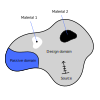
\includegraphics{figures/top_opt.png}}%%
    \caption{Topology optimization of a nanophotonic system, that is excited by an optical source. The simulation domain comprises a passive domain where the material is fixed, and a design domain (grey), where the material distribution is optimized for two different materials.}
        \label{fig:top_opt}
\end{figure}

For further details on inverse design by density-based topology optimization in photonics and nano-optics, we refer the reader to
the review papers by Jensen and Sigmund~\cite{jensen_review} and the more recent one by Molesky et al.~\cite{Molesky_2018}. 
For an introduction focusing on practical implementation, we refer the reader to the tutorial papers by Christiansen and Sigmund~\cite{tutorial_matlab, tutorial_COMSOL}.

\section{Structure of the thesis}

This thesis combines the concepts presented in \secref{intro:multi} and \secref{intro:to} by addressing multiphysics topology optimization problems in nanophotonics. The following chapters focus on reviewing
 the theoretical framework, presenting the contributions of this thesis in the context of state-of-the-art research,
  and concluding the thesis with a discussion of challenges and future research directions.

  \textbf{Chapter 2} introduces the theoretical framework used throughout the thesis, including the mathematical formalism
  to describe the propagation of light in nanophotonic systems (\secref{sec:nanophotonics}), the basics for the numerical implementation of 
  finite element-based simulation tools (\secref{sec:fem}) and the theory behind inverse design by topology optimization in multiphysics systems (\secref{sec:topopt_theory}).
  
  \textbf{Chapter 3} focuses on thermo-optically coupled topology optimization problems, emphasizing the topology optimization of 
  thermo-optical phase-shifters (\secref{sec:TOPS})~\cite{ownpub0}.
  
  \textbf{Chapter 4} addresses optomechanically coupled topology optimization problems, highlighting the optimization of optical forces via
  the Maxwell stress tensor formalism (\secref{sec:engi})~\cite{ownpub2}, integrated optical trapping cavities (\secref{sec:dip})~\cite{ownpub1, ownpub3}, and strongly coupled topology optimization 
  problems such as optomechanical membrane devices (\secref{sec:mech_strongly_coupled})~\cite{ownpub5}.
  
  \textbf{Chapter 5} explores electro-optically coupled topology optimization problems, with special focus on on the topology optimization of 
  nanolaser devices (\secref{sec:laser})~\cite{ownpub4}.
  
  \textbf{Chapter 6} concludes the thesis by summarizing the main results and outlining future work in the field of multiphysics topology optimization in nanophotonics.

This thesis consists of a collection of papers, including unpublished work on
strongly coupled optomechanical systems. The published and unpublished content is included in the attached
papers~\cite{ownpub0, ownpub1, ownpub2, ownpub3} and manuscripts~\cite{ownpub4, ownpub5}, respectively.
\openright
\chapter{Theoretical framework}

This chapter covers the theoretical foundations to understand the contents of this thesis, 
and is divided in four main sections. The first section presents the fundamental physics
governing optical problems, in the singlek physics picture. The second section provides 
an introduction to solving optical problems numerically using the finite-element method.
The third section introduces the concept of coupled optical systems, in the multi-physics
picture. The fourth section discusses the topology optimization of multi-physics systems.
With these tools we can understand how to solve the inverse design problems in the following
chapter.

%\begin{figure}[tb]
%    \centering
%    \makebox[\textwidth][c]{\includegraphics[width=1\imwidth]{figures/simpModel.png}}%
%    \caption{Bla bla bla...}
%    \label{fig:illustateTopOpt}
%\end{figure}


%\begin{equation}
%    (EIu'')'' = q
%\end{equation}


%\begin{figure}[tb]
%    \centering
%    \makebox[\textwidth][c]{\begin{tikzpicture}[remember picture]
    \begin{scope}[xshift=0mm]
        % angle (deg)
        \newcommand\ai{10}
        % line width
        \newcommand\wi{1pt}
        % cell size
        \newcommand\cellsize{3}
        % Rank-$N$ size
        \newcommand\di{0.75}

        % cell
        \draw[gray!10,   fill=gray!10, rotate around={\ai:(0,0)}] (0,0) rectangle (\cellsize,\cellsize) node (rect1) {};
        \draw[black!60, fill=black!60, rotate around={\ai:(0,0)}] (0,0) rectangle (\di,\cellsize);

        % orientation frame
        \draw[black, -stealth, line width=\wi, rotate around={\ai:({\di*cos(\ai) - \cellsize/2*sin(\ai)},{\di*sin(\ai) + \cellsize/2*cos(\ai)})}] ({\di*cos(\ai) - \cellsize/2*sin(\ai)},{\di*sin(\ai) + \cellsize/2*cos(\ai)}) -- ({\di*cos(\ai) - \cellsize/2*sin(\ai) + 0.75},{\di*sin(\ai) + \cellsize/2*cos(\ai)});
        \draw[black, -stealth, line width=\wi, rotate around={\ai:({\di*cos(\ai) - \cellsize/2*sin(\ai)},{\di*sin(\ai) + \cellsize/2*cos(\ai)})}] ({\di*cos(\ai) - \cellsize/2*sin(\ai)},{\di*sin(\ai) + \cellsize/2*cos(\ai)}) -- ({\di*cos(\ai) - \cellsize/2*sin(\ai)},{\di*sin(\ai) + \cellsize/2*cos(\ai) + 0.75});

        % local frame
        \draw[black, -stealth, dashed, line width=\wi] (0,0) -- ({\cellsize + 0.8},0);
        \draw[black, -stealth, dashed, line width=\wi] (0,0) -- (0,{\cellsize + 0.8});

        % ruler
        \draw[black, |-|, line width=\wi, rotate around={\ai:(0,0)}] (0,0) -- (\cellsize,0);
        \draw[black,  -|, line width=\wi, rotate around={\ai:(0,0)}] (0,0) -- (\di,0);

        % arc
        \draw[black, dotted, line width=\wi] (\cellsize,0) arc (0:\ai:\cellsize);

        % annotation
        \draw (\cellsize + 0.7, -0.3) node {$x_1 / \epsilon^3$};
        \draw (-0.5, \cellsize + 0.8) node {$x_2 / \epsilon^3$};
        \draw (\cellsize/2,-0.75) node {Rank-$1$};

        \draw[rotate around={{\ai/2}:(0,0)}] ({\cellsize+0.3},0) node {$\theta_1$};

        \draw[rotate around={{\ai}:(0,0)}] ({\di/2},0.4) node [rotate around={{\ai}:(0,0)}] {$\mu_1$};
        \draw[rotate around={{\ai}:(0,0)}] ({(\cellsize - \di)/2 + \di},0.4) node [rotate around={{\ai}:(0,0)}] {$1-\mu_1$};

        \draw[rotate around={{\ai}:(0,0)}] ({0+0.4},{\cellsize-0.4}) node [rotate around={{\ai}:(0,0)}] {$(+)$};
        \draw[rotate around={{\ai}:(0,0)}] ({\cellsize-0.4},{\cellsize-0.4}) node [rotate around={{\ai}:(0,0)}] {$(-)$};
        \coordinate (A) at (rect1.north);


        \draw[rotate around={\ai:({\di*cos(\ai) - \cellsize/2*sin(\ai)},{\di*sin(\ai) + \cellsize/2*cos(\ai)})}] ({\di*cos(\ai) - \cellsize/2*sin(\ai)+1} , {\di*sin(\ai) + \cellsize/2*cos(\ai) + 0.2}) node {$\mathbf{n}_1$};
        \draw[rotate around={\ai:({\di*cos(\ai) - \cellsize/2*sin(\ai)},{\di*sin(\ai) + \cellsize/2*cos(\ai)})}] ({\di*cos(\ai) - \cellsize/2*sin(\ai) + 0.3} , {\di*sin(\ai) + \cellsize/2*cos(\ai) + 1}) node {$\mathbf{m}_1$};



    \end{scope}
    \begin{scope}[xshift=45mm]
        % angle (deg)
        \newcommand\ai{15}
        % line width
        \newcommand\wi{1pt}
        % cell size
        \newcommand\cellsize{3}
        % Rank-$N$ size
        \newcommand\di{0.6}

        % cell
        \draw[gray!40,   fill=gray!40, rotate around={\ai:(0,0)}] (0,0) rectangle (\cellsize,\cellsize) node (rect2) {};
        \draw[black!60, fill=black!60, rotate around={\ai:(0,0)}] (0,0) rectangle (\di,\cellsize);

        % orientation frame
        \draw[black, -stealth, line width=\wi, rotate around={\ai:({\di*cos(\ai) - \cellsize/2*sin(\ai)},{\di*sin(\ai) + \cellsize/2*cos(\ai)})}] ({\di*cos(\ai) - \cellsize/2*sin(\ai)},{\di*sin(\ai) + \cellsize/2*cos(\ai)}) -- ({\di*cos(\ai) - \cellsize/2*sin(\ai) + 0.75},{\di*sin(\ai) + \cellsize/2*cos(\ai)});
        \draw[black, -stealth, line width=\wi, rotate around={\ai:({\di*cos(\ai) - \cellsize/2*sin(\ai)},{\di*sin(\ai) + \cellsize/2*cos(\ai)})}] ({\di*cos(\ai) - \cellsize/2*sin(\ai)},{\di*sin(\ai) + \cellsize/2*cos(\ai)}) -- ({\di*cos(\ai) - \cellsize/2*sin(\ai)},{\di*sin(\ai) + \cellsize/2*cos(\ai) + 0.75});

        % local frame
        \draw[black, -stealth, dashed, line width=\wi] (0,0) -- ({\cellsize + 0.8},0);
        \draw[black, -stealth, dashed, line width=\wi] (0,0) -- (0,{\cellsize + 0.8});

        % ruler
        \draw[black, |-|, line width=\wi, rotate around={\ai:(0,0)}] (0,0) -- (\cellsize,0);
        \draw[black,  -|, line width=\wi, rotate around={\ai:(0,0)}] (0,0) -- (\di,0);

        % arc
        \draw[black, dotted, line width=\wi] (\cellsize,0) arc (0:\ai:\cellsize);

        % annotation
        \draw (\cellsize + 0.7, -0.3) node {$x_1 / \epsilon^2$};
        \draw (-0.5, \cellsize + 0.8) node {$x_2 / \epsilon^2$};
        \draw (\cellsize/2,-0.75) node {Rank-$2$};

        \draw[rotate around={{\ai/2}:(0,0)}] ({\cellsize+0.3},0) node {$\theta_2 + \pi/4$};

        \draw[rotate around={{\ai}:(0,0)}] ({\di/2},0.4) node [rotate around={{\ai}:(0,0)}] {$\mu_2$};
        \draw[rotate around={{\ai}:(0,0)}] ({(\cellsize - \di)/2 + \di},0.4) node [rotate around={{\ai}:(0,0)}] {$1-\mu_2$};

        \draw[rotate around={{\ai}:(0,0)}] ({0+0.4},{\cellsize-0.4}) node [rotate around={{\ai}:(0,0)}] {$(+)$};
        \draw[rotate around={{\ai}:(0,0)}] ({\cellsize-0.9},{\cellsize-0.4}) node [rotate around={{\ai}:(0,0)}] (B) {$(\text{Rank-1})$};
        \coordinate (B2) at (rect2.north);


        \draw[rotate around={\ai:({\di*cos(\ai) - \cellsize/2*sin(\ai)},{\di*sin(\ai) + \cellsize/2*cos(\ai)})}] ({\di*cos(\ai) - \cellsize/2*sin(\ai)+1} , {\di*sin(\ai) + \cellsize/2*cos(\ai) + 0.2}) node {$\mathbf{n}_2$};
        \draw[rotate around={\ai:({\di*cos(\ai) - \cellsize/2*sin(\ai)},{\di*sin(\ai) + \cellsize/2*cos(\ai)})}] ({\di*cos(\ai) - \cellsize/2*sin(\ai) + 0.3} , {\di*sin(\ai) + \cellsize/2*cos(\ai) + 1}) node {$\mathbf{m}_2$};


    \end{scope}
    \begin{scope}[xshift=90mm]
        % angle (deg)
        \newcommand\ai{20}
        % line width
        \newcommand\wi{1pt}
        % cell size
        \newcommand\cellsize{3}
        % Rank-$N$ size
        \newcommand\di{1.0}

        % cell
        \draw[gray!60,   fill=gray!60, rotate around={\ai:(0,0)}] (0,0) rectangle (\cellsize,\cellsize);
        \draw[black!60, fill=black!60, rotate around={\ai:(0,0)}] (0,0) rectangle (\di,\cellsize);

        % orientation frame
        \draw[black, -stealth, line width=\wi, rotate around={\ai:({\di*cos(\ai) - \cellsize/2*sin(\ai)},{\di*sin(\ai) + \cellsize/2*cos(\ai)})}] ({\di*cos(\ai) - \cellsize/2*sin(\ai)},{\di*sin(\ai) + \cellsize/2*cos(\ai)}) -- ({\di*cos(\ai) - \cellsize/2*sin(\ai) + 0.75},{\di*sin(\ai) + \cellsize/2*cos(\ai)});
        \draw[black, -stealth, line width=\wi, rotate around={\ai:({\di*cos(\ai) - \cellsize/2*sin(\ai)},{\di*sin(\ai) + \cellsize/2*cos(\ai)})}] ({\di*cos(\ai) - \cellsize/2*sin(\ai)},{\di*sin(\ai) + \cellsize/2*cos(\ai)}) -- ({\di*cos(\ai) - \cellsize/2*sin(\ai)},{\di*sin(\ai) + \cellsize/2*cos(\ai) + 0.75});

        % local frame
        \draw[black, -stealth, dashed, line width=\wi] (0,0) -- ({\cellsize + 0.8},0);
        \draw[black, -stealth, dashed, line width=\wi] (0,0) -- (0,{\cellsize + 0.8});

        % ruler
        \draw[black, |-|, line width=\wi, rotate around={\ai:(0,0)}] (0,0) -- (\cellsize,0);
        \draw[black,  -|, line width=\wi, rotate around={\ai:(0,0)}] (0,0) -- (\di,0);

        % arc
        \draw[black, dotted, line width=\wi] (\cellsize,0) arc (0:\ai:\cellsize);

        % annotation
        \draw (\cellsize + 0.7, -0.3) node {$x_1 / \epsilon$};
        \draw (-0.5, \cellsize + 0.8) node {$x_2 / \epsilon$};
        \draw (\cellsize/2,-0.75) node {Rank-$3$};

        \draw[rotate around={{\ai/2}:(0,0)}] ({\cellsize+0.3},0) node {$\theta_3 - \pi/2$};

        \draw[rotate around={{\ai}:(0,0)}] ({\di/2},0.4) node [rotate around={{\ai}:(0,0)}] {$\mu_3$};
        \draw[rotate around={{\ai}:(0,0)}] ({(\cellsize - \di)/2 + \di},0.4) node [rotate around={{\ai}:(0,0)}] {$1-\mu_3$};

        \draw[rotate around={{\ai}:(0,0)}] ({0+0.4},{\cellsize-0.4}) node [rotate around={{\ai}:(0,0)}] {$(+)$};
        \draw[rotate around={{\ai}:(0,0)}] ({\cellsize-0.9},{\cellsize-0.4}) node [rotate around={{\ai}:(0,0)}] (C) {$(\text{Rank-2})$};


        \draw[rotate around={\ai:({\di*cos(\ai) - \cellsize/2*sin(\ai)},{\di*sin(\ai) + \cellsize/2*cos(\ai)})}] ({\di*cos(\ai) - \cellsize/2*sin(\ai)+1} , {\di*sin(\ai) + \cellsize/2*cos(\ai) + 0.2}) node {$\mathbf{n}_3$};
        \draw[rotate around={\ai:({\di*cos(\ai) - \cellsize/2*sin(\ai)},{\di*sin(\ai) + \cellsize/2*cos(\ai)})}] ({\di*cos(\ai) - \cellsize/2*sin(\ai) + 0.3} , {\di*sin(\ai) + \cellsize/2*cos(\ai) + 1}) node {$\mathbf{m}_3$};

    \end{scope}
    \path[-latex,black,thick] (A) edge [bend left=50] (B);
    \path[-latex,black,thick] (B2) edge [bend left=50] (C);
\end{tikzpicture}}%
%    \caption{Bla bla bla...}
%    \label{fig:Rank}
%\end{figure}

\section{Nano-optics -- Light as an electromagnetic wave}

In classical optics, light is treated as an electromagnetic (EM) wave, which can be described by 
solving Maxwell's equations. Solving these partial differential equations can be complicated, and 
depending on the characteristic size ($s$) of objects compared to the light's wavelength ($\lambda$) 
simpler limiting cases can be used to describe optical phenomena:
\begin{itemize}
    \item \textbf{Ray Optics ($s \ll \lambda$):} When objects are much larger than the wavelength, light is modeled as straight-line rays.
    \item \textbf{Quasistatics \& lumped circuit models ($s \gg \lambda$):} When objects are much smaller than the wavelength, the wave natue of light dissapears, 
    and can be approximated quasistatically (i.e., solving Poisson's equation). For instance, electronic devices can be modeled in this regime using circuit models w
    ith lumped elements, like resistors or capacitors. 
\end{itemize}
In the fields of photonics and \emph{nano-optics}, where the visible 
(\(\lambda \sim 400\)--\(800\) nm) and infrared (\(\lambda \sim 800\)--\(2500\) nm)
 spectral regions are most commonly explored, components often have nano- to
  microscale dimensions. As a result, we are in the \textbf{wave-optics} regime ($\lambda \sim s$ ),  
  where we cannot resort to simpler models like ray optics or quasistatic/lumped circuits models,
  and instead need to solve Maxwell's equations. Given the complexity of Maxwell's
  equations very few problems (e.g., problems with high symmetry, separability, few parameters) 
  can be solved analytically and for most problems requires 
  numerical solutions (e.g., the finite element method).


\subsection*{The macroscopic Maxwell's equations}

Light propagation in a \emph{macroscopic} electromagnetic systems can be described by Maxwell's equations. The time-domain Maxwell's 
equations in a linear, isotropic, and homogeneous medium can be written as:

\begin{align}
    \nabla \times \bm{\mathcal{E}} (\mathbf{r},t) &= - \frac{\partial \bm{\mathcal{B}}(\mathbf{r},t)}{\partial t}, \quad \quad &\text{(Faraday's law)} \label{eq:faraday}\\
    \nabla \times \bm{\mathcal{H}} (\mathbf{r},t) &= \frac{\partial \bm{\mathcal{D}}(\mathbf{r},t)}{\partial t} + \bm{\mathcal{J}}(\mathbf{r},t), \quad \quad &\text{(Ampère's law)} \label{eq:ampere}\\
    \nabla \cdot \bm{\mathcal{D}} (\mathbf{r},t) &= \mathcal{\rho}(\mathbf{r},t), \quad \quad &\text{(Gauss's law for electricity)} \label{eq:gauss_E}\\
    \nabla \cdot \bm{\mathcal{B}} (\mathbf{r},t) &= 0, \quad \quad &\text{(Gauss's law for magnetism)} \label{eq:Gauss_B}
\end{align}
where $\bm{\mathcal{E}}$ and $\bm{\mathcal{H}}$ are the time-dependent electric and magnetic (induction) fields, respectively, 
$\bm{\mathcal{D}}$ is the time-dependent electric displacement field,  
$\bm{\mathcal{B}}$ is the time-dependent magnetic (flux-density) field, $\bm{\mathcal{J}}$ is the current density,
and $\mathcal{\rho}$ is the time-dependent charge density. Maxwell's equations combine previously established
physical laws, in 4 equations:
\begin{itemize}
    \item \textbf{Faraday's law} [Eq.~\eqref{eq:faraday}] describes how a time-varying magnetic field induces an electric field.
    \item \textbf{Ampère's law} [Eq.~\eqref{eq:ampere}] describes how a time-varying electric field and electric current density induce a magnetic field.
    \item \textbf{Gauss's law for electricity} [Eq.~\eqref{eq:gauss_E}] describes how electric charges create an electric field. 
    \item \textbf{Gauss's law for magnetism} [Eq.~\eqref{eq:Gauss_B}] states that there are no magnetic monopoles, and thus the magnetic field lines are closed loops.
\end{itemize}

Note that the mascroscopic fields in Maxwell's equations 
are spatial averages of the
microscopic fields, and the charge and current densities are continous in space and time.
For an atomic scale description of the electromagnetic fields, one can use the \emph{microscopic}
Maxwell's equations, which include a quantized description of matter based on discrete charged particles
(e.g., electrons, protons, etc.), and currents.\\

To understand how materials respond to electromagnetic fields,
we need to introduce the constitutive equations. These materials can be modeled
with the presence of a time-dependent polarization $\bm{\mathcal{P}}$ and magnetization $\bm{\mathcal{M}}$, 
which relate the fields $\bm{\mathcal{D}}$ and $\bm{\mathcal{B}}$ to the fields $\bm{\mathcal{E}}$ and 
$\bm{\mathcal{H}}$ by the constitutive equations:
\begin{align}
    \bm{\mathcal{D}}(\mathbf{r}, t) &= \varepsilon_0 \bm{\mathcal{E}}(\mathbf{r}, t) + \bm{\mathcal{P}}(\mathbf{r}, t), \label{eq:D}\\ 
    \bm{\mathcal{H}}(\mathbf{r}, t) &= \mu_0^{-1} \bm{\mathcal{B}}(\mathbf{r}, t) - \bm{\mathcal{M}}(\mathbf{r}, t) \label{eq:H},
\end{align}
where $\varepsilon_0$ is the permittivity of free space and $\mu_0$ is the permeability of free space. 
note that the polarization and magnetization also depend on the electric and magnetic fields; as an example the
polarization can be written as a series expansion in powers of the electric field: 
$\bm{\mathcal{P}}=\mathcal{\varepsilon}_0 \bm{\mathcal{\chi}}^{(1)} \bm{\mathcal{E}}+\mathcal{\varepsilon}_0 \bm{\mathcal{\chi}}^{(2)} \bm{\mathcal{E}} \bm{\mathcal{E}}+\mathcal{\varepsilon}_0 \bm{\mathcal{\chi}}^{(3)} \bm{\mathcal{E}} \bm{\mathcal{E}} \bm{\mathcal{E}}+\cdots$,
where $\bm{\mathcal{\chi}}^{n}$ is the $n^\text{th}$ order component of the electric susceptibility. In this thesis
we will only consider linear materials, where only the first-order terms in the expansion are considered. \\


Using Maxwell's equations and applying the curl operator to Faraday's law [Eq.~\eqref{eq:faraday}] and Ampère's law [Eq.~\eqref{eq:ampere}], 
together with the constitutive relations for $\mathbf{D}$ and $\mathbf{B}$ in Eq.~\eqref{eq:D} and Eq.~\eqref{eq:H}, one gets two coupled
wave equations for the electric and magnetic fields:
\begin{equation}
\begin{aligned}
    & \nabla \times \nabla \times \bm{\mathcal{E}}+\frac{1}{c^2} \frac{\partial^2 \bm{\mathcal{E}}}{\partial t^2}=-\mu_0 \frac{\partial}{\partial t}\left(\bm{\mathcal{J}}+\frac{\partial \bm{\mathcal{P}}}{\partial t}+\nabla \times \bm{\mathcal{M}}\right), \\
    & \nabla \times \nabla \times \bm{\mathcal{H}}+\frac{1}{c^2} \frac{\partial^2 \bm{\mathcal{H}}}{\partial t^2}=\nabla \times \bm{\mathcal{J}}+\nabla \times \frac{\partial \bm{\mathcal{P}}}{\partial t}-\frac{1}{c^2} \frac{\partial^2 \bm{\mathcal{M}}}{\partial t^2}
\end{aligned}
\end{equation}
where $c=(\varepsilon_0 \mu_0)^{-1/2}$ is the speed of light in vacuum. This equation described the wave nature of electromagnetic fields,
and is generally valid for any material.

\subsection*{Electromagnetics in the frequency domain}

The time-dependence in Maxwell's equations can be separated by assuming a harmonic time-dependence of the fields:
\begin{equation}
    \bm{\mathcal{E}}(\mathbf{r}, t) = \Re \{ \mathbf{E}(\mathbf{r}) e^{-i\omega t} \}= \frac{1}{2}\left[ \mathbf{E}(\mathbf{r}) e^{i\omega t} + \mathbf{E}^*(\mathbf{r}) e^{-i\omega t}\right],
\end{equation}
where $\mathbf{E}$ is the complex field phasor, $\omega=ck$ is the angular frequency of the light, and $k=2\pi/\lambda$ is the wavenumber.
Using this complex field, the time-domain Maxwell's equations can be written as
\begin{align}
    \nabla \times \mathbf{E}(\mathbf{r}) &= -i\omega \mathbf{B}(\omega, \mathbf{r}), \quad \quad &\text{(Faraday's law)} \label{eq:curlE_freq}\\
    \nabla \times \mathbf{H}(\mathbf{r}) &= i\omega  \mathbf{D}(\mathbf{r}) + \mathbf{j}(\mathbf{r}), \quad \quad &\text{(Ampère's law)} \label{eq:curlH_freq}\\
    \nabla \cdot \mathbf{D}(\mathbf{r}) &= \rho(\mathbf{r}), \quad \quad &\text{(Gauss's law for electricity)} \label{eq:divD_freq}\\
    \nabla \cdot \mathbf{B}(\mathbf{r}) &= 0, \quad \quad &\text{(Gauss's law for magnetism)} \label{eq:divB_freq}
\end{align}

where all fields now are complex phasors that also depend on the frequency
(e.g., $\mathbf{E}(\omega, \mathbf{r})$) and only have spatial dependence. In a similar fashion,
the material parameters are complex functions of space and frequency (e.g., $\varepsilon(\omega, \mathbf{r}$)). 
Note that the frequency-domain Maxwell's equations are equivalent to applying Fourier transform in time to the time domain
equations [Eqs.~\eqref{eq:faraday}-\eqref{eq:Gauss_B}].\\

By using the frequency-domain constitutive relations and applying the curl operator to Faraday's law [Eq.~\eqref{eq:curlE_freq}] and Ampère's law [Eq.~\eqref{eq:curlH_freq}],
we can combine both equations into a single wave equation for the electric field\footnote{A similar procedure one can be applied to derive a wave equation for the magnetic field.
}:

\begin{equation}
    \nabla \times \left(\frac{1}{\mu} \nabla \times \mathbf{E}\right) - k^2 \varepsilon \mathbf{E} = -i\omega \mu \mathbf{j}(\mathbf{r})\,. 
\end{equation}
This is the Helmholtz equation for the electric field. This equation can 
be further simplified by adopting an operator nomenclature:
\begin{empheq}[box={\fboxsep=5pt\fboxrule=0.5pt\fbox}]{equation}\label{eq:helmholtz}
    \mathcal{L}[\mathbf{E}(\mathbf{r})] = \mathbf{f}\,,
\end{empheq}
where $\mathcal{L} \triangleq \nabla \times \left[(1/\mu) \nabla \times \mathbf{\square} \right] - k^2 \square $ is a differential operator acting on a vector field $\mathbf{\square}$, 
and $\mathbf{f} = -i\omega \mu \mathbf{j}(\mathbf{r})$ is the source term. This equation is the cornerstone of the numerical analysis in this thesis.

\subsection*{Boundary conditions at material interfaces}

In many physical systems, and specially in computational optics, the medium can be divided
into different regions with different material properties. Although a piecewise homogeneous
medium is an inhomoegeneous medium, the inhomogeneities are confined to the boundaries and 
the optical problem can be solved in each region separately. The solutions to the optical problems
are connected by the boundary conditions at the interfaces between the regions; and thus between
materials. These boundary conditions can be derived from Maxwell's equations, and for a boundary
$\Gamma_{ij}$ separating domain $i$ from domain $j$ yield the tangential field conditions:
\begin{align}
    \mathbf{n} \times (\mathbf{E}_i - \mathbf{E}_j) &= 0 \label{eq:BC_E}\\
    \mathbf{n} \times (\mathbf{H}_i - \mathbf{H}_j) &= \mathbf{K} , \label{eq:BC_H}
\end{align} 
and the normal field conditions:
\begin{align}
    \mathbf{n} \cdot (\mathbf{D}_i - \mathbf{D}_j) &= \rho_s \label{eq:BC_D}\\
    \mathbf{n} \cdot (\mathbf{B}_i - \mathbf{B}_j) &= 0, \label{eq:BC_B}
\end{align}
where $\mathbf{n}$ is the normal vector to the boundary, $\mathbf{K}$ is the surface current density,
 and $\rho_s$ is the surface charge density. Note that In many optical problems there are no 
 sources in the individual domains, and $\mathbf{K}$ and $\rho$ are zero.

 LINK THIS TO THE NEDELEC ELEMENTS!

\subsection*{Modeling single emitters: the Green's function formalism}

\subsection*{Some useful properties of Maxwell's equations}
The following are some key properties of Maxwell's equations and the Helmholtz operator that will be useful throughout this thesis.:
\begin{itemize}
    \item \textbf{Linearity and superposition:} The operator introduced in Eq.~\eqref{eq:helmholtz} is linear, meaning the superposition principle holds. If $\mathbf{E}_1$ and $\mathbf{E}_2$ are t
    wo solutions to the Helmholtz equation, such that $\mathcal{L}[\mathbf{E}_1] = \mathbf{f}_1$ and 
    $\mathcal{L}[\mathbf{E}_2] = \mathbf{f}_2$, then their linear combination ($\mathbf{E}_3 = \alpha \mathbf{E}_1 + \beta \mathbf{E}_2$) 
    is also a solution:
    \begin{equation}
        \mathcal{L}[\mathbf{E}_3] = \mathcal{L}[\alpha \mathbf{E}_1 + \beta \mathbf{E}_2] = \alpha \mathcal{L}[\mathbf{E}_1] + \beta \mathcal{L}[\mathbf{E}_2] = \alpha \mathbf{f}_1 + \beta \mathbf{f}_2 = \mathbf{f}_3\,.
    \end{equation}
    For instance, if the source term is scaled by a proportionality factor, the resulting field solution will also be scaled by the same factor, maintaining the proportional relationship. 

    \item \textbf{Hermiticity:} The operator $\mathcal{L}$ is self-adjoint, meaning that the inner product of two solutions is invariant under the operator:
    \begin{equation}
        \int \mathbf{E}_1^* \cdot \mathcal{L}[\mathbf{E}_2] \d \mathbf{r} = \int \mathcal{L}[\mathbf{E}_1]^* \cdot \mathbf{E}_2 \d \mathbf{r}\,,
    \end{equation}
    This property ensures that purely real eigenvalues and orthogonal eigenmodes\footnote{Except for degenerate eigenmodes, which will not necessarily be orthogonal.}, as shown in \cite{phot_crys}. Moreover,
    one can show that the operator is \textbf{positive semi-definitive}, meaning that all eigenvalues ($k^2$) are non-negative. Since all eigenvalues are real and non-negative, the operator $\mathcal{L}$ is \textbf{diagonalizable}.
    RELATE TO SOLVER CHOICE LATER.
    
    \item \textbf{Scale-invariance:} The Helmholtz operator $\mathcal{L}(\mathbf{r})$ is invariant under a change of scale. 
    If $\mathbf{E}(\mathbf{r})$ is a solution to the Helmholtz equation for the frequency $\omega$, then $\mathbf{E}(\alpha \mathbf{r})$ 
    is also a solution for any scaling factor $\alpha$, given a constant
     dielectric permittivity $\varepsilon(\omega, \mathbf{r}) = \varepsilon (\omega^\prime, \alpha \mathbf{r})$ at a frequency $\omega^\prime = \alpha \omega$ \cite{phot_crys}. Similarly,
     if we scale the dielectric permittivity by a value $\alpha$ the electric field distribution is constant when working at a re-scaled version of the 
     frequency $\omega^\prime=\omega/\alpha $ \cite{phot_crys}.
    In other words, as long as the permittivity is constant under spatial transformations, there is no fundamental lengthscale or dielectric permittivity  
    values in mascroscopic electromagnetic systems. Note however, that in general the dielectric permittivity is a function of the frequency $\varepsilon(\omega)\neq \varepsilon(\omega^\prime)$, 
    breaking scale-invariance.
    
    \item \textbf{Conservation laws:} Maxwell's equations inherently satisfy several conservation laws, which are fundamental to physical systems MAKE SURE OF THE SYMBOLS AND EQUATIONS THEY ARE TIME-DOMAIN:
    \begin{itemize}
        \item \textbf{Charge conservation:} The continuity equation ensures that charge is conserved in the system:
        \begin{equation}
            \nabla \cdot \mathbf{J} + \frac{\partial \rho}{\partial t} = 0.
        \end{equation}
        This equation relates the divergence of the current density $\mathbf{J}$ to the time rate of change of the charge density $\rho$.

        \item \textbf{Energy conservation:} The Poynting theorem describes the conservation of electromagnetic energy:
        \begin{equation}
            \nabla \cdot \mathbf{S} + \frac{\partial u}{\partial t} = -\mathbf{J} \cdot \mathbf{E},
        \end{equation}
        where $\mathbf{S} = \mathbf{E} \times \mathbf{H}$ is the Poynting vector representing the energy flux, and $u = (1/2) (\varepsilon |\mathbf{E}|^2 + \mu |\mathbf{H}|^2)$ is the electromagnetic energy density.

        \item \textbf{Momentum conservation:} The electromagnetic fields carry momentum, and the conservation of momentum is described by the Maxwell stress tensor $\mathbf{T}$:
        \begin{equation}
            \nabla \cdot \mathbf{T} + \frac{\partial \mathbf{p}}{\partial t} = \mathbf{f},
        \end{equation}
        where $\mathbf{p}$ is the momentum density and $\mathbf{f}$ is the force density acting on the system. The electromagnetic fields also carry \textbf{angular momentum}, and its conservation is described by the angular momentum density $\mathbf{L}$:
                    \begin{equation}
                        \frac{\partial \mathbf{L}}{\partial t} + \nabla \cdot \mathbf{M} = \boldsymbol{\tau},
                    \end{equation}
                    where $\mathbf{M}$ is the angular momentum flux density tensor, and $\boldsymbol{\tau} = \mathbf{r} \times \mathbf{f}$ represents the torque density acting on the system.
    \end{itemize}
    
    \item \textbf{Time-reversal symmetry:} Maxwell's equations remain valid if we reverse the direction of time ($t\to-t$). It can be shown that under time-reversal symmetry
                                                the fields transform as $\bm{\mathcal{E}}(\mathbf{r}, t)\to\bm{\mathcal{E}}(\mathbf{r}, -t)$,  $\bm{\mathcal{D}}(\mathbf{r}, t)\to\bm{\mathcal{D}}(\mathbf{r}, -t)$,
                                                 $\bm{\mathcal{H}}(\mathbf{r}, t)\to-\bm{\mathcal{H}}(\mathbf{r}, -t)$, and $\bm{\mathcal{B}}(\mathbf{r}, t)\to-\bm{\mathcal{B}}(\mathbf{r}, -t)$, while the current density and charge density transform as 
                                                 $\bm{\mathcal{J}}(\mathbf{r}, t)\to-\bm{\mathcal{J}}(\mathbf{r}, -t)$ and $\bm{\mathcal{\rho}}(\mathbf{r}, t)\to\bm{\mathcal{\rho}}(\mathbf{r}, -t)$, respectively \cite{reciprocity}.
                                                 Applying these transformations to Maxwell's equations in Eqs. \eqref{eq:curlE_freq}-\eqref{eq:divB_freq} shows that the equations remain invariant under time-reversal. This 
                                                 symmetry can be extended by considering \textbf{Parity-time (PT) symmetry}, which combines time-reversal with spatial inversion ($\mathbf{r}\to-\mathbf{r}$) and is satisfied for materials with
                                                 $\varepsilon(\mathbf{r}) = \varepsilon^*(-\mathbf{r})$ and $\mu(\mathbf{r}) = \mu^*(-\mathbf{r})$. There are however some situations where time-reversal symmetry and/or PT symmetry is broken, 
                                                 such as in the presence of non-reciprocal materials (e.g., magneto-optical materials) or materials with optical losses \cite{ownpub0}.VERIFY AND CITE SOME PT SYMMETRY PAPER.
        
    \item \textbf{Reciprocity:} In an optical system the source and the detector of electromagnetic fields can be interchanged without changing the physical situation. Let's consider a system where two volumes $\Omega_1$ and $\Omega_2$ 
    have two current densities $\mathbf{j}_1$ and $\mathbf{j}_2$ that create the fields $\mathbf{E}_1$, $\mathbf{H}_1$ and $\mathbf{E}_2$, $\mathbf{H}_2$ respectively. Using the Lorentz recirpocity theorem one can show that \cite{novotny}:      
    \begin{equation}
        \int_{\Omega_1} \mathbf{E}_1^* \cdot \mathbf{j}_2 = \int_{\Omega_2}  \mathbf{E}_2^* \cdot \mathbf{j}_1 d\mathbf{r} = 0.
    \end{equation}
    For losless media this is equivalent to time-reversal symmetry, but for lossy systems reciprocity still remains valid \cite{Carminati:98}. Reciprocity is a very useful property of Maxwell's equations, as it can be used to 
    greatly simplify some formulations of inverse design problems [CITE LASER PAPER].


\end{itemize}

\subsection*{Point-like emitters: the Green's function formalism}

TODO: Add if we do coupled-emitter project.

\section{The finite element method in electromagnetics}

(CHECK IANS THESIS)

The weak form of the wave equation can be written as (CHECK CHATGPT):
\begin{equation}
    \int_{\Omega} \nabla \times \mathbf{E} \cdot \nabla \times \mathbf{v} - k^2 \int_{\Omega} \mathbf{E} \cdot \mathbf{v} = \int_{\Omega} \mathbf{J} \cdot \mathbf{v} \quad \forall \mathbf{v} \in V,
\end{equation}
The weak form can be discretized by using the finite-element method. An example is shown in Figure YY, 
where we have discretized the two-dimensional domain in Figure XX into a set of triangular edge elements. 
The edge elements, or Nedelec elements (CITE), of first kind are a natural choice for the electromagnetic 
wave equation, as they are divergence-free and enforce the continuity of the tangential electric field 
across the element boundaries, which is a natural boundary condition for Maxwell's equations 
\footnote{For 2D models where the field discontinuity at the material interfaces 
is in the out-of-plane direction (e.g., Publication 3), one can use Lagrange element without 
exciting spurious modes.}. In Figure YY
we show the structure of a Nedelec element alongside a quiver plot of the shape function one of the edges.
Using the shape functions we can calculate the contribution of the different elements to the weak form of the
wave equation, which can be assembled into a system of equations in the strong form:
\begin{equation}
    \mathbf{K} \mathbf{E} = \mathbf{F},
\end{equation}
where $\mathbf{K}$ is the stiffness matrix, $\mathbf{E}$ is the electric field, and $\mathbf{F}$ is the source
 term. In the case of eigenvalue problems the source term is zero ($\mathbf{F}=0$), and the system of equations 
that needs to be solved is given by:
\begin{equation}
    \left(\mathbf{K} - \lambda \mathbf{I} \right) \mathbf{E} =  \mathbf{0},
\end{equation}

Note that the stiffness matrix is symmetric indefinite, restricting the use of iterative solvers (e.g., Cholesky factorization, Krylov method) to solve the system of equations. Instead LU factorization is a common choice for direct solvers.
\begin{figure}[tb]
    \centering
    \makebox[\textwidth][c]{
\includegraphics{figures/FEM.png}}%%
    \caption{Geometrical discretization of the physical domain into the finite element mesh, which is composed of Nedelec vector-elements. The element colored in light blue is a triangular element with three nodes and three edges, where we have sketched a quiver plot for the shape function $\mathbf{N}_2$ for Edge 2.}
    \label{fig:fem}
\end{figure}

Eigenvalue vs RHS problems


Lagrange elements vs Edge elements. Comment spurious modes.

Symmetry conditions can be applied to reduce the computational
cost of the solutions by employing perfect electric conductor (PEC) and perfect magnetic 
conductor (PMC) boundary conditions. The PEC boundary condition
imposes symmetry for magnetic fields and antisymmetry for electric fields and electric 
currents, by setting the tangential component of the electric field to zero: $\mathbf{n}\times \mathbf{E} = 0$ .
The PMC boundary condition imposes symmetry for electric fields and antisymmetry for magnetic fields
by setting the normal component of the magnetic field to zero: $\mathbf{n}\cdot \mathbf{H} = 0$.

\section{Beyond single-physics -- coupled optical systems}

Coupled multi-physics systems are physical systems where the solution of one of the physical 
problem depends on the solution of another physical problem. Let's consider that the two
problems can be described by linear partial differential equations, where the first problem
is described by the equation $\mathcal{L}_1 [\mathbf{u}]= \mathbf{a}$ and the second problem is described by the 
equation $\mathcal{L}_2 [\mathbf{w}]= \mathbf{b}$.

 If this relation is unidirectional
we call it \textbf{weak coupling}, and if the relation is bidirectional we call it 
\textbf{strong coupling}.

In weaky coupled systems, both physical problems can be solved independently in a seggregated 
manner, where the solution of one problem is used in the the other problem.

In strongly coupled systems, the physical problems are solved simultaneously.

Differentiate between weak and strong coupling.

\section{Topology optimization of multiphysics systems}

\begin{equation}
    \begin{array}{clr}
    \max\limits_{\xi} & \Phi(\xi, \mathbf{u}) & \text { (Objective function) } \\
    \text { s.t. } & \mathbf{S}_i(\xi, \mathbf{u})-\mathbf{f}_i=0 \quad \forall i \in\left[1, N_S\right] & \text { (State equations) } \\
    & c_j(\xi, \mathbf{u}) \leq 0 \quad \forall j \in\left[1, N_c\right] & \text { (Inequality constraints) } \\
    & \xi_{\text {min }} \leq \xi \leq \xi_{\text {max }} & \text { (Box constraints) }
    \end{array}
\end{equation}

The optimization problem is solved using the algorithm of the Method of Moving
Asymptotes (MMA) (CITE) and Globally Convergent Method of Moving Ssymptotes (GCMMA) (CITE).

\subsection{From densities to material properties}

To regularize the optimization and introduce a weak sense of geometric length scale, we filter
the density field using a filter operation. The filtered density can be calculated using a 
convolution-based filter operation (CITE)
\begin{equation}
    \begin{aligned}
    & \tilde{\xi}(\mathbf{r})=\frac{\sum_{k \in \mathcal{B}_{e, h}} w\left(\mathbf{r}-\mathbf{r}_k\right) A_k \xi_k}{\sum_{k \in \mathcal{B}_{e, h}} w\left(\mathbf{r}-\mathbf{r}_k\right) A_k}, \\
    & w(\mathbf{r})=\left\{r_f-|\mathbf{r}| \quad \forall|\mathbf{r}| \leq r_f, \quad r_f \geq 0, \quad \mathbf{r} \in \Omega\right.\,,
    \end{aligned}
\end{equation}

where $A_k$ is the area of the kth element, and $\mathcal{B}_{e, h}$ denotes the
$h^\text{th}$ set of finite elements whose center point is within a filter radius $r_f$ of the
$h^\text{th}$ element. One can also filter by solving a Helmholtz-type PDE (CITE):
\begin{equation}
    -\left(\frac{r_f}{2 \sqrt{3}}\right)^2 \nabla \tilde{\xi}+\tilde{\xi}=\xi
\end{equation}
The filter operation is followed by a smoothed Heaviside threshold:
\begin{equation}
    \bar{\tilde{\xi}}=\frac{\tanh (\beta \cdot \eta)+\tanh (\beta \cdot(\tilde{\xi}-\eta))}{\tanh (\beta \cdot \eta)+\tanh (\beta \cdot(1-\eta))}, \quad \beta \in[1, \infty[, \eta \in[0,1],
\end{equation}
where $\beta$ and $\eta$ control the threshold sharpness and value, respectively.

The physical field cna be interpolated to the filtered density field using a material interpolation.
In multi-physics problems, we will have one material interpolation for each different physical problem
\footnote{If the problem stem from the same physics (e.g., solving two optical problems), the material interpolation can be re-used.}.
In general, the material interpolation can be written as:
\begin{equation}
    \zeta(\bar{\tilde{\xi}})=\zeta_0+\bar{\tilde{\xi}}^p\left(\zeta_1-\zeta_0\right)
\end{equation}
where $\zeta$ is the material property, $\zeta_0$ and $\zeta_1$ are the material properties of the void and solid, respectively, and $p$
is a penalization factor (usually, $p=3$ for compliance optimization and $p$=1 for other problems). Note that for some
special cases, like optical optimization problems with metals, it is benefitial to employ a non-linear material interpolation.

Do it in such a way that it works for multiphysics.
Invert order of threshold and filter operations.

\subsection{Adjoint sensitivity analysis}

(CHECK NIELS THESIS)

The adjoint sensitivity analysis is used to efficiently calculate the gradient of the objective function with 
respect to the design variables. In this thesis, we use the adjoint sensitivity analysis  in the context of 
multi-physics problems, where multiple complex-valued PDE are solved. Let us rewrite the FOM by adding the residual
of the state equation and its complex conjugate, multiplied by the Lagrange multipliers, $\lambda_i$ and $\lambda_{i+N}$, 
respectively:
\begin{equation}
    \tilde{\Phi} =\Phi + \sum^N_i \left[ \lambda_{i}^{\top}\left(\mathbf{S}_i \mathbf{u}^*_i -\mathbf{f}_i\right) + 
    \lambda_{i+N}^{\dagger}\left(\mathbf{S}_{i}^* \mathbf{u}^*_i -\mathbf{f}_i^*\right) \right]
\end{equation}

\subsubsection*{Coupled source problems}

\subsubsection*{Coupled state-equation problems}


\section{A practical note on computational implementation}

Using first order edge, or nodal, elements a rule of thumb is to include at least 10 elements per wavelength.

Discuss direct vs iterative solvers, discuss condition number of the system.
Sparsity, symmetry, definitiness
Discuss the practical implementation, with COMSOL and other means (Fenics, gridap, etc).
Check Niels, Ian's thesis, and other references.
Bla bla bla...
\openright
\chapter{Thermo-optical topology optimization problems}
%CHECK COPYRIGHT FOR FIGURES AND REPRINTS
%In this chapter we will focus on the effects of multiphysics couplings in nanophotonic devices, reviewing state-of-the-art research, 
%highlighting open topology optimization problems, and presenting our contributions to the field.
%We will focus on three main classes of multiphysics couplings: thermo-optical, opto-mechanical, and electro-optical systems.
%\begin{figure}[tb]
%    \centering
%    \makebox[\textwidth][c]{\includegraphics[width=1\imwidth]{figures/simpModel.png}}%
%    \caption{Bla bla bla...}
%    \label{fig:illustateTopOpt}
%\end{figure
%\begin{equation}
%    (EIu'')'' = q
%\end{equation}
%\beginfigure}[tb]
%    \centering
%    \makebox[\textwidth][c]{\begin{tikzpicture}[remember picture]
    \begin{scope}[xshift=0mm]
        % angle (deg)
        \newcommand\ai{10}
        % line width
        \newcommand\wi{1pt}
        % cell size
        \newcommand\cellsize{3}
        % Rank-$N$ size
        \newcommand\di{0.75}

        % cell
        \draw[gray!10,   fill=gray!10, rotate around={\ai:(0,0)}] (0,0) rectangle (\cellsize,\cellsize) node (rect1) {};
        \draw[black!60, fill=black!60, rotate around={\ai:(0,0)}] (0,0) rectangle (\di,\cellsize);

        % orientation frame
        \draw[black, -stealth, line width=\wi, rotate around={\ai:({\di*cos(\ai) - \cellsize/2*sin(\ai)},{\di*sin(\ai) + \cellsize/2*cos(\ai)})}] ({\di*cos(\ai) - \cellsize/2*sin(\ai)},{\di*sin(\ai) + \cellsize/2*cos(\ai)}) -- ({\di*cos(\ai) - \cellsize/2*sin(\ai) + 0.75},{\di*sin(\ai) + \cellsize/2*cos(\ai)});
        \draw[black, -stealth, line width=\wi, rotate around={\ai:({\di*cos(\ai) - \cellsize/2*sin(\ai)},{\di*sin(\ai) + \cellsize/2*cos(\ai)})}] ({\di*cos(\ai) - \cellsize/2*sin(\ai)},{\di*sin(\ai) + \cellsize/2*cos(\ai)}) -- ({\di*cos(\ai) - \cellsize/2*sin(\ai)},{\di*sin(\ai) + \cellsize/2*cos(\ai) + 0.75});

        % local frame
        \draw[black, -stealth, dashed, line width=\wi] (0,0) -- ({\cellsize + 0.8},0);
        \draw[black, -stealth, dashed, line width=\wi] (0,0) -- (0,{\cellsize + 0.8});

        % ruler
        \draw[black, |-|, line width=\wi, rotate around={\ai:(0,0)}] (0,0) -- (\cellsize,0);
        \draw[black,  -|, line width=\wi, rotate around={\ai:(0,0)}] (0,0) -- (\di,0);

        % arc
        \draw[black, dotted, line width=\wi] (\cellsize,0) arc (0:\ai:\cellsize);

        % annotation
        \draw (\cellsize + 0.7, -0.3) node {$x_1 / \epsilon^3$};
        \draw (-0.5, \cellsize + 0.8) node {$x_2 / \epsilon^3$};
        \draw (\cellsize/2,-0.75) node {Rank-$1$};

        \draw[rotate around={{\ai/2}:(0,0)}] ({\cellsize+0.3},0) node {$\theta_1$};

        \draw[rotate around={{\ai}:(0,0)}] ({\di/2},0.4) node [rotate around={{\ai}:(0,0)}] {$\mu_1$};
        \draw[rotate around={{\ai}:(0,0)}] ({(\cellsize - \di)/2 + \di},0.4) node [rotate around={{\ai}:(0,0)}] {$1-\mu_1$};

        \draw[rotate around={{\ai}:(0,0)}] ({0+0.4},{\cellsize-0.4}) node [rotate around={{\ai}:(0,0)}] {$(+)$};
        \draw[rotate around={{\ai}:(0,0)}] ({\cellsize-0.4},{\cellsize-0.4}) node [rotate around={{\ai}:(0,0)}] {$(-)$};
        \coordinate (A) at (rect1.north);


        \draw[rotate around={\ai:({\di*cos(\ai) - \cellsize/2*sin(\ai)},{\di*sin(\ai) + \cellsize/2*cos(\ai)})}] ({\di*cos(\ai) - \cellsize/2*sin(\ai)+1} , {\di*sin(\ai) + \cellsize/2*cos(\ai) + 0.2}) node {$\mathbf{n}_1$};
        \draw[rotate around={\ai:({\di*cos(\ai) - \cellsize/2*sin(\ai)},{\di*sin(\ai) + \cellsize/2*cos(\ai)})}] ({\di*cos(\ai) - \cellsize/2*sin(\ai) + 0.3} , {\di*sin(\ai) + \cellsize/2*cos(\ai) + 1}) node {$\mathbf{m}_1$};



    \end{scope}
    \begin{scope}[xshift=45mm]
        % angle (deg)
        \newcommand\ai{15}
        % line width
        \newcommand\wi{1pt}
        % cell size
        \newcommand\cellsize{3}
        % Rank-$N$ size
        \newcommand\di{0.6}

        % cell
        \draw[gray!40,   fill=gray!40, rotate around={\ai:(0,0)}] (0,0) rectangle (\cellsize,\cellsize) node (rect2) {};
        \draw[black!60, fill=black!60, rotate around={\ai:(0,0)}] (0,0) rectangle (\di,\cellsize);

        % orientation frame
        \draw[black, -stealth, line width=\wi, rotate around={\ai:({\di*cos(\ai) - \cellsize/2*sin(\ai)},{\di*sin(\ai) + \cellsize/2*cos(\ai)})}] ({\di*cos(\ai) - \cellsize/2*sin(\ai)},{\di*sin(\ai) + \cellsize/2*cos(\ai)}) -- ({\di*cos(\ai) - \cellsize/2*sin(\ai) + 0.75},{\di*sin(\ai) + \cellsize/2*cos(\ai)});
        \draw[black, -stealth, line width=\wi, rotate around={\ai:({\di*cos(\ai) - \cellsize/2*sin(\ai)},{\di*sin(\ai) + \cellsize/2*cos(\ai)})}] ({\di*cos(\ai) - \cellsize/2*sin(\ai)},{\di*sin(\ai) + \cellsize/2*cos(\ai)}) -- ({\di*cos(\ai) - \cellsize/2*sin(\ai)},{\di*sin(\ai) + \cellsize/2*cos(\ai) + 0.75});

        % local frame
        \draw[black, -stealth, dashed, line width=\wi] (0,0) -- ({\cellsize + 0.8},0);
        \draw[black, -stealth, dashed, line width=\wi] (0,0) -- (0,{\cellsize + 0.8});

        % ruler
        \draw[black, |-|, line width=\wi, rotate around={\ai:(0,0)}] (0,0) -- (\cellsize,0);
        \draw[black,  -|, line width=\wi, rotate around={\ai:(0,0)}] (0,0) -- (\di,0);

        % arc
        \draw[black, dotted, line width=\wi] (\cellsize,0) arc (0:\ai:\cellsize);

        % annotation
        \draw (\cellsize + 0.7, -0.3) node {$x_1 / \epsilon^2$};
        \draw (-0.5, \cellsize + 0.8) node {$x_2 / \epsilon^2$};
        \draw (\cellsize/2,-0.75) node {Rank-$2$};

        \draw[rotate around={{\ai/2}:(0,0)}] ({\cellsize+0.3},0) node {$\theta_2 + \pi/4$};

        \draw[rotate around={{\ai}:(0,0)}] ({\di/2},0.4) node [rotate around={{\ai}:(0,0)}] {$\mu_2$};
        \draw[rotate around={{\ai}:(0,0)}] ({(\cellsize - \di)/2 + \di},0.4) node [rotate around={{\ai}:(0,0)}] {$1-\mu_2$};

        \draw[rotate around={{\ai}:(0,0)}] ({0+0.4},{\cellsize-0.4}) node [rotate around={{\ai}:(0,0)}] {$(+)$};
        \draw[rotate around={{\ai}:(0,0)}] ({\cellsize-0.9},{\cellsize-0.4}) node [rotate around={{\ai}:(0,0)}] (B) {$(\text{Rank-1})$};
        \coordinate (B2) at (rect2.north);


        \draw[rotate around={\ai:({\di*cos(\ai) - \cellsize/2*sin(\ai)},{\di*sin(\ai) + \cellsize/2*cos(\ai)})}] ({\di*cos(\ai) - \cellsize/2*sin(\ai)+1} , {\di*sin(\ai) + \cellsize/2*cos(\ai) + 0.2}) node {$\mathbf{n}_2$};
        \draw[rotate around={\ai:({\di*cos(\ai) - \cellsize/2*sin(\ai)},{\di*sin(\ai) + \cellsize/2*cos(\ai)})}] ({\di*cos(\ai) - \cellsize/2*sin(\ai) + 0.3} , {\di*sin(\ai) + \cellsize/2*cos(\ai) + 1}) node {$\mathbf{m}_2$};


    \end{scope}
    \begin{scope}[xshift=90mm]
        % angle (deg)
        \newcommand\ai{20}
        % line width
        \newcommand\wi{1pt}
        % cell size
        \newcommand\cellsize{3}
        % Rank-$N$ size
        \newcommand\di{1.0}

        % cell
        \draw[gray!60,   fill=gray!60, rotate around={\ai:(0,0)}] (0,0) rectangle (\cellsize,\cellsize);
        \draw[black!60, fill=black!60, rotate around={\ai:(0,0)}] (0,0) rectangle (\di,\cellsize);

        % orientation frame
        \draw[black, -stealth, line width=\wi, rotate around={\ai:({\di*cos(\ai) - \cellsize/2*sin(\ai)},{\di*sin(\ai) + \cellsize/2*cos(\ai)})}] ({\di*cos(\ai) - \cellsize/2*sin(\ai)},{\di*sin(\ai) + \cellsize/2*cos(\ai)}) -- ({\di*cos(\ai) - \cellsize/2*sin(\ai) + 0.75},{\di*sin(\ai) + \cellsize/2*cos(\ai)});
        \draw[black, -stealth, line width=\wi, rotate around={\ai:({\di*cos(\ai) - \cellsize/2*sin(\ai)},{\di*sin(\ai) + \cellsize/2*cos(\ai)})}] ({\di*cos(\ai) - \cellsize/2*sin(\ai)},{\di*sin(\ai) + \cellsize/2*cos(\ai)}) -- ({\di*cos(\ai) - \cellsize/2*sin(\ai)},{\di*sin(\ai) + \cellsize/2*cos(\ai) + 0.75});

        % local frame
        \draw[black, -stealth, dashed, line width=\wi] (0,0) -- ({\cellsize + 0.8},0);
        \draw[black, -stealth, dashed, line width=\wi] (0,0) -- (0,{\cellsize + 0.8});

        % ruler
        \draw[black, |-|, line width=\wi, rotate around={\ai:(0,0)}] (0,0) -- (\cellsize,0);
        \draw[black,  -|, line width=\wi, rotate around={\ai:(0,0)}] (0,0) -- (\di,0);

        % arc
        \draw[black, dotted, line width=\wi] (\cellsize,0) arc (0:\ai:\cellsize);

        % annotation
        \draw (\cellsize + 0.7, -0.3) node {$x_1 / \epsilon$};
        \draw (-0.5, \cellsize + 0.8) node {$x_2 / \epsilon$};
        \draw (\cellsize/2,-0.75) node {Rank-$3$};

        \draw[rotate around={{\ai/2}:(0,0)}] ({\cellsize+0.3},0) node {$\theta_3 - \pi/2$};

        \draw[rotate around={{\ai}:(0,0)}] ({\di/2},0.4) node [rotate around={{\ai}:(0,0)}] {$\mu_3$};
        \draw[rotate around={{\ai}:(0,0)}] ({(\cellsize - \di)/2 + \di},0.4) node [rotate around={{\ai}:(0,0)}] {$1-\mu_3$};

        \draw[rotate around={{\ai}:(0,0)}] ({0+0.4},{\cellsize-0.4}) node [rotate around={{\ai}:(0,0)}] {$(+)$};
        \draw[rotate around={{\ai}:(0,0)}] ({\cellsize-0.9},{\cellsize-0.4}) node [rotate around={{\ai}:(0,0)}] (C) {$(\text{Rank-2})$};


        \draw[rotate around={\ai:({\di*cos(\ai) - \cellsize/2*sin(\ai)},{\di*sin(\ai) + \cellsize/2*cos(\ai)})}] ({\di*cos(\ai) - \cellsize/2*sin(\ai)+1} , {\di*sin(\ai) + \cellsize/2*cos(\ai) + 0.2}) node {$\mathbf{n}_3$};
        \draw[rotate around={\ai:({\di*cos(\ai) - \cellsize/2*sin(\ai)},{\di*sin(\ai) + \cellsize/2*cos(\ai)})}] ({\di*cos(\ai) - \cellsize/2*sin(\ai) + 0.3} , {\di*sin(\ai) + \cellsize/2*cos(\ai) + 1}) node {$\mathbf{m}_3$};

    \end{scope}
    \path[-latex,black,thick] (A) edge [bend left=50] (B);
    \path[-latex,black,thick] (B2) edge [bend left=50] (C);
\end{tikzpicture}}%
%    \caption{Bla bla bla...}
%    \label{fig:Rank}
%\end{figure}
%\section{Coupled optical systems}
%TODO: Include if we end up doing the Green's function study.
% Make a connection to the Green's function formalism and derive system of coupled equations.
%\section{Thermo-optical systems~\cite{ownpub0}}\label{sec:thermo_optical}
Thermo-optical systems exploit the interplay between the temperature and electromagnetic fields to enable active control over optical properties. 
The main mechanism behind this coupling is the thermo-optic effect, 
in which the refractive index of a material changes as a function of temperature. 
This effect plays a central role in many integrated photonics application; such as,
 optical phase shifters~\cite{TOPS_1, TOPS_2, TOPS_3}, reconfigurable photonic circuits~\cite{program, PIC}, and thermally tunable switches~\cite{switch, switch_2} and filters~\cite{filter}.

 Despite its wide usage, optimizing thermo-optical devices remains challenging due to the intricate coupling 
 between thermal and optical physics. Topology optimization offers a systematic design optimization solution, with application examples in
  thermo-optical phase shifters~\cite{TOPS_heat, ownpub0}, optical mirror-like thermo-mechanical structures~\cite{opt_perf}, and
structural integrity constraints~\cite{structural_heat}, among others.

In the following sections, we summarize how to model and optimize thermo-optic systems, 
with special focus on our research contribution~\cite{ownpub0}, which to the best of our knowledge,
extends the state-of-the art uncoupled and single-physics thermo-optic topology optimization frameworks by, for the first time, considering 
the coupled physical problem.

\section{The thermo-optic effect}

To model the coupled thermo-optical topology optimization problem, we combine the governing equation of the optical model (\eqref{eq:wave_eq})
with a heat transfer model. The simplest heat trasfer model is the steady-state heat equation, which describes the
heat transfer in a medium due to conduction and heat sources. The \textbf{heat equation} is given by
\begin{equation}\label{eq:heat}
    -\nabla \cdot \left[ \kappa(\mathbf{r})\cdot \nabla T(\mathbf{r}) \right] = Q(\mathbf{r})
\end{equation}
where $T$ is the temperature, $\kappa$ is the thermal conductivity, and $Q$ is a volumetric heat source. Note that this equation can be
extended by consider convection and radiation effects, which may be important in some thermo-optical systems (see the boundary conditions
in~\cite{ownpub0}).

Temperature can be coupled to the optical response via the \textbf{thermo-optic coefficient} (TOC), which links the temperature field
with the refractive index of the material, typically approximated with the linear relation\footnote{Large temperature gradients may lead to nonlinear effects, requiring higher order terms.}
\begin{equation}
n(\mathbf{r}) = n_0 + \text{TOC} \cdot \left[T(\mathbf{r}) - T_0\right],
\end{equation}
where $n_0$ and $T_0$ are the reference (unheated) refractive index and reference temperature, respectively. Thus, to solve a problem coupled throught the TOC, one first solves the heat equation
to determine the temperature profile, which can be used to determine
the spatially varying refractive index, which is then used in \eqref{eq:wave_eq} to determine the optical field.

\section{Topology optimization of thermo-optical phase-shifters~\cite{ownpub0}}\label{sec:TOPS}

Among the many applications that utilize the thermo-optic coefficient, we find integrated photonic circuit components, which rely on the large 
TOC of silicon ($\text{TOC} \approx 1.8 \cdot 10^{-4}\, \text{K}^{-1}$) at room-temperature ($\approx300$ K) and telecom wavelength 
($\lambda=1.55$ \textmu m)~\cite{thermo-optic-coef}. One of those components is the thermo-optical phase shifter, which, as shown in \figref{fig:thermo_opt},
uses a heating device to locally modify the refractive index of a waveguide structure to induce a \textbf{phase shift} ($\Delta \Phi$) in the propagating optical mode
\begin{equation*}
\Delta \Phi = \frac{2\pi L}{\lambda} \Delta n_\text{eff},
\end{equation*}
where $L$ is the device length and $\Delta n_\text{eff} = n_\text{eff, heated} - n_\text{eff, unheated}$ is the change of the effective index of the waveguide. 

\subsection*{The effective index via waveguide finite-element analysis}

In order to calculate the phase-shift one thus needs to find the effective index of an optical mode, which can be done by 
using the finite-element formulation for two-dimensional waveguide cross-sections~\cite{jin}:
\begin{equation}\label{eq:wg_eq}
    \left[\begin{array}{cc}
    A_{\text{tt}}(\varepsilon,k) & 0 \\
    0 & 0
    \end{array}\right]
    \left\{\begin{array}{l}
    E_{\text{t}} \\
    E_z
    \end{array}\right\}
    = -k_z^2
    \left[\begin{array}{cc}
    B_{\text{tt}} & B_{\text{t} z} \\
    B_{z \text{t}} & B_{z z}(\varepsilon,k)
    \end{array}\right]
    \left\{\begin{array}{c}
    E_{\text{t}} \\
    E_z
    \end{array}\right\},
    \end{equation}
where $E_{\text{t}}$ and $E_z$ are the transverse and longitudinal electric field components, $k_z$ is the propagation constant of the optical mode, and $A_{tt}, B_{tt},
B_{zt}$ and $B_{tz}$ are matrices that can be assembled using the interpolation functions. Following~\cite{jin}, we use first-order Nédélec elements for in-plane components and 
second-order Lagrange elements for out-of-plane components\footnote{Lagrange elements must be one order higher than edge elements to properly represent gradients or curls.}. 
Solving the generalized eigenvalue problem in \eqref{eq:wg_eq} yields waveguide modes ($E_t$, $E_z$) and propagation constants ($k_z$). The propagation constant can be rewritten into the effective index $n_\text{eff} = k_z / k$,
 where the real part is a measure of the mode overlap with the refractive index distribution, and the imaginary part ($\Im\{n_\text{eff}\}$) quantifies optical losses. 

 \subsection*{PT-symmetry breaking waveguides}

Recent progress in waveguide design by U.D. Dave and M. Lipson~\cite{lipson}, proposed the use of PT-symmetry breaking waveguides as good canditates for
thermo-optical phase shifters, since they can minimize optical losses near (lossy) metallic heaters. To understand this phenomenon we solve the generalized
eigenvalue problem in \eqref{eq:wg_eq} for a waveguide where half of the core is lossy (characterized by $\Im\{n\}>0$).  As loss increases, the fundamental mode becomes more lossy until reaching an (exceptional) 
point where it bifurcates into high- and low-loss modes. Surprisingly, further increasing $\Im\{n\}$ counter-intuitively reduces the loss of the low-loss mode. This effect is particularly useful in the design of
thermo-optical waveguide devices, since it enables to position a lossy metallic heater in direct contact with the waveguide core, while the mode is still able to propagate with low losses.

\begin{figure}[tb]
    \centering
    \makebox[\textwidth][c]{\includegraphics{figures/TOPS_pt.png}}%%
    \caption{Parity-time symmetry breaking and interpretation of losses of propagating modes. Make this figure look better.}
    \label{fig:thermo_opt}
\end{figure}

\subsection*{Topology optimization results~\cite{ownpub0}}

Inspired by PT-symmetry breaking waveguides, in~\cite{ownpub0} we use topology optimization to have good heat conduction and low optical loss in thermo-optical phase shifters.
The optimization problem considers a waveguide cross-section with a metallic heater, and seeks to minimize optical loss in an optical waveguide for both heated and 
unheated configurations. Unlike the eigenvalue-based approach in~\cite{lipson}, in this work we evaluate losses by solving a linear system of equations where we excite the waveguide 
and calculate the excited mode's 
amplitude. As illustrated in \figref{fig:thermo_opt}, maximizing the mode amplitude, is equivalent minimizing the width of the effective 
index resonance, and thus the loss of the mode. Based on this insight, we formulate the optimization problem, where we design the metalic heater around the waveguide, by using a worst-case maximization 
of the electric-field intensity at two effective indices corresponding to heated and unheated 
waveguide configurations. To integrate the heat problem into the topology optimization framework we use a linear material interpolation 
for the conductivity and an interpolation for the heat source
\begin{equation}
    Q(\hat{\rho})=P_{\text{in}} \frac{\hat{\rho}^p}{L a_e \sum_j \hat{\rho}_j}\,,
\end{equation}
where $P_\text{in}$ is the input power in the heater, $p=3$ is a penalization factor, and $a_e$ is the area of the element. With these interpolations we can solve a design-dependent
heat problem which then is fed into the optical problem to calculate the amplitude of the unheated and heated modes. To solve the inverse design
problem we derive a coupled adjoint sensitivity analysis, as further detailed in~\cite{ownpub0}, enabling the use of gradient-based optimization. CHECK AND
MENTION IF THE OPTIMIZE DEVICES RELY ON THE PT-SYMMETRY BREAKING EFFECT. COMMENT ON IT.

Using this framework we find the results in \figref{fig:thermo_res}, where we depict the optimized waveguide cross-section with a metallic heater, which is able to homogeneously heat the waveguide core,
allowing the same low-loss mode to propagate in both the heated and unheated scenarios. Moreover, several extensions of the topology optimization problem are considered for varying volume constraints, optical power, and including fabrication constraints (e.g., minimum lengthscales, and layered 
litography processes). SAY HOW MucH IMPROVEMENT WE GOT!

\begin{figure}[tb]
    \centering
    \makebox[\textwidth][c]{\includegraphics{figures/TOPS_results.png}}%%
    \caption{Topology optimization of thermo-optical phase-shifters. (a) Phase-shifting mechanism, where a heater changes the temperature in the waveguide $\Delta T$, which for a length $L$ creates a phase-shift
    $\Delta \Phi$. (b) Thermal and optical response of the topology optimized device. Adapted with permission from~\cite{ownpub0} \copyright Optical Society of America.}
    \label{fig:thermo_res}
\end{figure}

\subsection*{Outlook and future work}

The framework laid out in our work~\cite{ownpub0} opens up the avenue for the study and optimization to weakly coupled topology optimization problems. For example, for the design of phase-shifters and thermo-optical modulators, it should be straightforward to extend this
formalism to three dimensional system, where one could account for insertion/coupling losses of the integrated photonic circuits. Another example could be the to use multi-material topology optimization, to design not-only the heating
device, but also the optical waveguide. Finally, this formalism could be applied to design completely different devices, such as re-configurable photonic systems that might be modulated by an external heat source, or thermo-optical
switches based on optical cavities~\cite{switch, switch_2}, where the change in refractive index shifts the cavity in- or out-of-resonance.

SAY THAT CONDUCTION AND ELECTROSTATICS ARE SIMILAR CITE POCKELS PAPER AND TALK ABOUT ELECTRO-OPTICAL MODULATION!

\section{Towards strong coupling -- heat dissipation in optics}\label{sec:thermo_strong_coupling}

In the strong coupling regime, the optical response will modify the thermal response, and vice versa.
For example, optical absorption can lead to significant local heating, altering the refractive index and modifying the optical field. 
This mutual dependence requires strongly a coupled treatment of the heat and optical problems, 
which can be accounted for by modeling the optical absorption with an electric field dependent volumetric heat source~\cite{plasm_heat_source}
\[
Q(\mathbf{r}) = \frac{1}{2} \omega \varepsilon_0 \operatorname{Im}[\varepsilon(\mathbf{r})] |\mathbf{E}(\mathbf{r})|^2,
\]
where the material losses ($\Im[\varepsilon]$) convert the electromagnetic energy into heat. 
This expression is particularly important in metal nanostructures, where plasmonic resonances can lead to localized temperature increases~\cite{plasm_heat_source}, or in 
high-intensity photonics where even low absorption materials can generate significant heat~\cite{thermal_nl, high_I_T}. Moreover, the thermo-optical feedback can give rise to nonlinear effects, such as self-focusing~\cite{thermal_nl}. As a matter of fact, if we still consider a linear
thermal response and thermo-optico coefficient,
the nonlinearity has the form of a Kerr-type nonlinearity ($\Delta n \propto \vert \mathbf{E} \vert^2$). Accouting and modeling
these effects could open up the avenue for the inverse design of novel nonlinear thermophotonic devices, with potential applications
in integrated nonlinear photonics~\cite{nl_photonics}, metasurfaces~\cite{nl_meta} and plasmonics~\cite{novotny}.


\section{Heat transfer as an auxiliary connectivity constraint}

Lastly, it is worthwile mentioning that the heat equation can be used as an auxiliary equation to enforce connectivity
and structural integrit in topology optimization problems~\cite{vanessa, structural_heat}, which is employed in several of our
works~\cite{ownpub1,ownpub2}. 

This method, introduced in~\cite{li_structural_2016}, is known as the Virtual Temperature
Method (VTM). The core idea of the VTM is to simulate a heat transfer problem on an auxiliary thermal field, where the design 
domain is treated as a heat source and a thermally conductive material, while void regions are modeled as an
insulating material, and a Dirichlet boundary condition ($T = 0$) is imposed on the boundaries where connectivity is required. When 
solving the steady-state heat equation [\eqref{eq:heat}], regions that are disconnected from the boundary 
cannot dissipate heat and therefore attain elevated temperatures. By applying a threshold criterion such as $T < T_\text{thresh}$, disconnected islands in the design can be 
detected and penalized. For instance, in our works~\cite{ownpub1,ownpub2} we compute a measure of the total virtual temperature
by integrating the temperature field over the design domain, and add it as a constraint in the optimization problem:
$\int_{\Omega_D} T \d \Omega \leq \epsilon_C$, where $\Omega_D$ is the design domain and $\epsilon_c$ is sufficiently small constant. This ensures that the final design remains physically connected to the required 
boundaries. 


Note that by appropriately selecting the connecting boundaries it is possible to use the VTM to enforce
structural integrity of the designs~\cite{structural_heat}, although this can also be ensured by solving an auxiliary
mechanical problem~\cite{structural_integrity}. For a more robust connectivity constraint formulation with less parameter tuning (e.g., material conductivies) we refer the reader to the Nonlinear 
Virtual Temperature Method (NVTM)~\cite{nvtm}, and for further details on connectivity constraints we refer the reader to the review 
article by Cool et al.~\cite{vanessa}.

\openright
\chapter{Optomechanical topology optimization problems}
%\section{Opto-mechanical systems~\cite{ownpub1,ownpub2,ownpub3}}\label{sec:optomechanics}
Optomechanics, the study of the interaction between light and mechanical motion, is at the heart of state-of-the-art technologies, such as 
optical trapping~\cite{ashkin_acceleration_1970, moffitt_recent_2008} and cooling~\cite{cooling}, quantum information processing~\cite{Andrews_2014, Xi_2025}
, light sails~\cite{lightsail, lightsail1}, and high-precision metrology and sensing~\cite{sensing, weakforce, Li:18, Mason_2019}.

The most basic description of this interaction is given by the Lorentz force, which governs how moving charges respond to electric and magnetic fields:
\begin{equation}\label{eq:lorentz_f}
    \mathbf{\bm{\mathcal{F}}}(\mathbf{r},t) = q \left[ \bm{\mathcal{E}}(\mathbf{r},t) + \mathbf{v}(t) \times \bm{\mathcal{B}}(\mathbf{r},t) \right]\,,
\end{equation}
where $q$ is the charge and $\mathbf{v}$ is the velocity of the particle. This force can be generalized to describe more complex systems,
such as the the force between two current-carrying 
wires (Ampere's force law), and the electromotive force, which is at the core of many techologies, such as induction motors or generators.
In optomechanical systems, shaping the distribution and magnitude of these forces at the micro- and nanoscale is crucial for controlling mechanical motion with light. 
However, designing structures that can efficiently harness and manipulate these interactions often requires navigating highly complex
 parameter spaces and trade-offs between optical, mechanical, and material constraints.

To achieve such precise control, topology optimization has emerged as a a useful design technique enhance or tailor optomechanical interactions.
Recent advances include the design of coupling between optical and elastic
 waves~\cite{photo_topopt}, optical systems with nonlinear deformations~\cite{def_wg}, high-$Q$ optomechanical membranes~\cite{highQ1, fengwen, aragon1},
light sail structures~\cite{lightsail_topopt, lightsail_topopt1},
on-chip optical trapping devices~\cite{ownpub1}, particle design and manipulation~\cite{ownpub2, particle_opt},
and structural integrity constraint formulations~\cite{structural_integrity}
 among others.

 In the following subsections, we highlight our contributions to the field and review how to model optomechanical interactions in three distinct regimes: a general treatment based on the Maxwell stress tensor~\cite{ownpub2}; 
 the dipole approximation for small particles~\cite{ownpub1, ownpub3}; and strongly coupled systems where optical forces can induce significant mechanical deformations.
\section{The Maxwell Stress Tensor formalism~\cite{ownpub3}}

In the most-general case, the optical force can be calculated using the Maxwell stress tensor (MST) formalism, which can be derived from the generalization of the Lorentz force (\eqref{eq:lorentz_f}) in continuous media~\cite{novotny}.
The basic idea is sketched in \figref{fig:eng_res}, where
a particle scatters an incident electromagnetic field $\mathbf{E}_\text{inc}$ creating the scattered field $\mathbf{E}_\text{scat}$ and the net force $\mathbf{F}$ that acts
on the particle. The time-averaged net force is given by
\begin{equation}\label{eq:f_MST}
    \langle\bm{\mathcal{F}}\rangle=\int_{\partial V}\langle\stackrel{\leftrightarrow}{\bm{\mathcal{T}}}(\mathbf{r}, t)\rangle \cdot \mathbf{n}_{\partial V}(\mathbf{r}) \d \mathbf{r}\,,
\end{equation}
where $\partial V$ denotes any boundary enclosing the particle, $n_{\partial V}$ denotes the unitary vector normal to that boundary, and
the stress tensor is given by:
\begin{equation}
    \begin{aligned}
        \stackrel{\leftrightarrow}{\bm{\mathcal{T}}}(\mathbf{r}, t)= & {\left[\varepsilon_0 \varepsilon_r \mathcal{E}(\mathbf{r}, t) \otimes \mathcal{E}(\mathbf{r}, t)+\mu_0 \mu_r \mathcal{H}(\mathbf{r}, t) \otimes \mathcal{H}(\mathbf{r}, t)\right.} \\
    & \left.-\frac{1}{2}\left(\varepsilon_0 \varepsilon_r \mathcal{E}^2(\mathbf{r}, t)+\mu_0 \mu_r \mathcal{H}^2(\mathbf{r}, t)\right) \stackrel{\leftrightarrow}{\mathbf{I}}\right],
    \end{aligned}
\end{equation}
where $\otimes$ denotes the outer product. Note that the permittivity and permeability correspond to those of the medium surrounding the particle.

\begin{figure}[tb]
    \centering
    \makebox[\textwidth][c]{\includegraphics{figures/eng_results.png}}%%
    \caption{Topology optimization in optical force applications. (a) A scattering particle 
    enclosed by a boundary $\partial V$ scatters a field $\mathbf{E}_\text{scat}$, when excited by an incident field $\mathbf{E}_\text{inc}$, 
    generating a net optical force $\mathbf{F}$. (b) Electric-field intensity distribution for a particle design optimized to maximize the vertical ($y$)
    component of the optical force. Adapted with permission from~\cite{ownpub2} \copyright Optical Society of America.}
    \label{fig:eng_res}
\end{figure}

\subsection*{Engineering optical forces via topology optimization}

In~\cite{ownpub3} we use this formalism to optimize the geometry of particle-metalens pairs for difference applications, such as attracting, repelling, 
oscillating and trapping particles. In \figref{fig:eng_res} we depict an example optimization result from our work, where 
we optimize the geometry of a particle to maximize the vertical component of the optical force by maximizing $\text{FOM} = \langle\bm{\mathcal{F}}\rangle \cdot \mathbf{n}_y$, where
in our two-dimensional example $\mathbf{n}_y = (0, 1)$ is the unitary vector in the vertical direction.  Our results show that the optimized particle geometry is a Bragg-mirror-like
structure, which is able to efficiently reflecting the incoming plane-wave, resulting in a efficient exchange of force and momentum. In the remainder of~\cite{ownpub3} we extend this example by also designign a metalens to focus the incoming plane-wave onto the particle,
we design attractive particle geometries, and optical-tweezer like setups to trap the particle in space. All the code developed in this work is available on GitHub~\cite{github_MST} with examples on force calculation and topology optimization. 

One interesting aspect of the topology optimization of particles in the MST formalism is that with our current framework the particle cannot feature disconnected members; otherwise
one would need to integrate around the individual components to calculate the total force for each one. It is possible to get around this by enforcing 
a connectivity constraint via the VTM~\cite{li_structural_2016}(see \secref{sec:thermo_optical}). In our examples
we enforce particle connectivity to the center of the design domain, and also of the metalens structure to the bottom, as to ensure Structural
integrity of the structure.

\subsection*{Outlook and future work}

This optimization work is the first, to our knowledge, to 
consider the MST formalism, paving the way for future work in three-dimensional systems and more complex optimization problems, such as optically-driven particle
trajectory control~\cite{zemanek_perspective_2019, macdonald_microfluidic_2003, shilkin_directional_2017}, many-body particle systems~\cite{bechinger_active_2016, chang_colloquium_2018} or optically actuated devices~\cite{ivanyi_optically_2024}, among others.
Finally, it is worth noting that a particularly interesting and straightforward extension would be to use the MST formalism to calculate the time-averaged torque acting on a particle, defined as~\cite{novotny}
\begin{equation}
    \langle \bm{\tau} \rangle = \langle \mathbf{r} \times \bm{\mathcal{F}} \rangle = \int_{\partial V} \langle \mathbf{r}
     \times \stackrel{\leftrightarrow}{\bm{\mathcal{T}}} \rangle \cdot \mathbf{n}_{\partial V} \d\mathbf{r} 
\end{equation}
where $\mathbf{r}$ is the vector defimed between the rotation axis and force application point. This definition of torque accounts
for two kinds of rotational motion; \textit{spinning} ($\langle \bm{\tau}_S \rangle$), where the particle rotates around its center of mass,
and \textit{orbiting} ($\langle \bm{\tau}_O \rangle$), where the particle rotates around an external axis, so that the total torque is the sum
of both the spin and orbital torque $\langle \bm{\tau} \rangle = \langle \bm{\tau}_S \rangle + \langle \bm{\tau}_O \rangle$~\cite{torque}.  Defining
and optical torque-based FOM could open the door for the design of efficient optical and biological micro- and nanomachines~\cite{rotating}.

\section{The dipole approximation~\cite{ownpub1, ownpub3}}

When particles are much smaller than the wavelength of the electromagnetic field ($s\ll \lambda$), it is possible to model the optical force via the dipole approximation in the
quasistatic limit. In this approximation, the particle is treated as a point dipole with a polarizability $\alpha$, which describes how the particle responds to the local electric field frequency-domain $\mathbf{E}$.
In the dipole approximation the optical force on the particle can be expressed as~\cite{novotny}:
\begin{equation}
    \langle\mathbf{F}\rangle=\overbrace{\frac{\alpha^{\prime}}{4} \nabla\left\{\mathbf{E}^* \cdot \mathbf{E}\right\}}^{(1)}
    +\frac{\alpha^{\prime \prime}}{k \varepsilon_0} \Big[\overbrace{\frac{1}{c}\langle \mathbf{S} \rangle}^{(2)} + \overbrace{c \left( \nabla \times \langle \mathbf{L} \rangle \right)}^{(3)}\Big]\,,
\end{equation}
where the polarizability can be split up into the real and imaginary parts 
$\alpha=\alpha^\prime + i \alpha^{\prime \prime}$, the Poynting vector is given by $\mathbf{S} = \mathbf{E} \times \mathbf{H}$, and the time-averaged angular momentum is 
$\langle \mathbf{L} \rangle = [\varepsilon_0/(4 i \omega)](\mathbf{E} \times \mathbf{E}^*)$. 
The term associated with the Poynting vector is the radiation pressure ($2$), while the term associated 
with the angular momentum ($3$) is the spin-curl force.

In the abscence of absorption effects ($\alpha^{\prime \prime}=0$), the force is totally described 
by the gradient force ($1$), which is a conservative force that can be described as the gradient 
of a trapping potential:
\begin{equation*}
    U (\mathbf{r}) = -\frac{\alpha^{\prime}}{4} \left|\mathbf{E}(\mathbf{r})\right|^2\,.
\end{equation*}
where the force can be calculated as $\mathbf{F} = -\nabla U(\mathbf{r})$. 
For non-resonant and non-absorbing isotropic particles the polarizability is 
described through the relation~\cite{BornWolf:1999:Book}
\begin{equation}
    \alpha^{\prime}= 3 \varepsilon_0 $V$ \frac{\varepsilon_p-\varepsilon_m}{\varepsilon_p+2 \varepsilon_m}\,,
\end{equation}
where $V$ is the volume of the particle, $\varepsilon_p$ and $\varepsilon_m$ are the
dielectric constants of the particle and the medium, respectively. Note that in the dipole approximation do not consider the particle modifying
the optical field, which works well for point-like particles in free-space but not necessarily 
for either large particles, particles with high refractive contrast, or particles close to material
boundaries (e.g., optical cavities). This interaction can be accounted for in the dipole
approximation by considering the self-induced back-action (SIBA) effect, which assumes a weak
perturbation of the field due to the particle and expands the field in terms of 
the scattering Green function of the particle, which leads to a self-consistent
equation for the total electric field which can be used to calculate the force~\cite{novotny, SIBA, benjamin}. If the series converges this leads 
to same result as the MST calculation (\eqref{eq:f_MST}), which is often used to validate the dipole approximation (e.g., \cite{ownpub1,ownpub3}). 

\subsection*{On-chip omnidirectional optical trapping via topology optimization~\cite{ownpub1}}

Using the dipole approximation formalism in~\cite{ownpub1} we use topology optimization to design an integrated omnidirectional optical trapping chip, which is able to trap particles in three dimensions,
which was previously only possible with the use of free-space optical tweezers~\cite{ashkin_acceleration_1970}, or bulky photonic devices~\cite{manka_simulation_2024}. This is done by minimizing 
the difference of the electric-field norm with respect to a reference field $\mathbf{E}_\text{ref}$:
\begin{equation}
    \text{FOM} \equiv \Phi=\sqrt{\int_{\Omega}\left[\Theta\left(\frac{|\mathbf{E}(\mathbf{r})|}{\left|\mathbf{E}\left(\mathbf{r}_0\right)\right|}-\frac{\left|\mathbf{E}_{\text{ref}}(\mathbf{r})\right|}{\left|\mathbf{E}_{\text{ref}}\left(\mathbf{r}_0\right)\right|}\right)\right]^2} \text{~d} \Omega
    \end{equation}
where the fields are normalized with respect to the value at the center of the design domain $\mathbf{r}_0$, and $\Theta$ is the smoothed Heaviside threshold, which ensures
potentials as steep or steeper than the reference. The reference is chosen as a Gaussian trapping potential, but can be any other potential, such as a harmonic potential ($U\propto\mathbf{r}^2$).

By applying this optimization framework we obtain the topology-optimized cavity design in \figref{fig:MST_dipole}, which is able to trap particles at the center of an optical
cavity in three dimensions and has an associated Gaussian-like trapping potential, with a depth  $U<-10\, k_B T$ at room temperature ($T=300$ K) conventionally needed to overcome Brownian fluctuations~\cite{novotny}.
As long as the dipole approximation is valid one can tune the input power to trap paricles of arbitrarily small sizes.

\begin{figure}[tb]
    \centering
    \makebox[\textwidth][c]{\includegraphics{figures/MST_dipole.png}}%%
    \caption{Optical response and trappig potential for the topology-optimized particle trap. (a) Lower half ($z<0$) of the optimized cavity, with the electric-field intensity
    distribution when excited with the fundamental waveguide mode at $\lambda=1.55$ \textmu m. (b) Trapping potential for a $R=15$ nm and $n=2$ particle in the cavity region for the different axial line- and plane-cuts as a function
    of the distance from the center ($d$), with the stable trapping regime ($U<-10 k_B\, T$) highlighted in gray. Adapted with permission from~\cite{ownpub1}.}
    \label{fig:MST_dipole}
\end{figure}

From the dipole approximation trapping potential we calculate the the force-displacements curves and we determine trapping stiffnesses
of $\kappa \approx 0.5$ fN/nm, an order of magnitude larger that diffraction-limited free-space optical tweezers~\cite{ownpub1}. To validate this findings
we employ the MST formalism to calculating the force on spherical particles as they are displaced from the cavity center in the axial directions, and find excellent
agreement with the dipole approximation. As shown in \figref{fig:SPIE}, to further verify the the dipole approximation assumption in ~\cite{ownpub3} we compare the results of the dipole approximation with the MST
for varying particle sizes and refractive indices, showing that the dipole approximation is a good approximation
even for large values of the refractive index (e.g., $n=3$) and particle sizes up to $s\approx 0.05 \lambda$. As we can see for larger sizes and refractive indices 
the results start to deviate, and the dipole approximation should break down for even larger values.

\begin{figure}[tb]
    \centering
    \makebox[\textwidth][c]{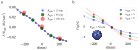
\includegraphics{figures/SPIE_results.png}}%%
    \caption{Validating the dipole approximation force (dashed line) against the MST force (data points), for the force as a function of displacement ($d$) from the cavity center.
    (a) Volume-normalized force ($F/R^2_\text{sph}$) for different particle sizes with refractive index $n_\text{sph}=2$. (b) Force for different refractive indices of the particle for a particle radius $R_\text{sph}=50$ nm. Adapted from~\cite{ownpub3}.}
    \label{fig:SPIE}
\end{figure}

\subsection*{Benchmarking trapping performance~\cite{ownpub1}}

When designing optical trapping platforms it is important to be able to compare performance across platforms. To this end, in~\cite{ownpub3} we introduce a normalized
trapping stiffness metric, which normalizes trapping stiffness to particle  polarizability and input power ($P_\text{in}$)
\begin{equation}
    \eta_i=\frac{\kappa_i \varepsilon_0}{\alpha^\prime P_{\text{in}}}
\end{equation}
enabling one-to-one comparison across trapping devices\footnote{As noted in~\cite{ownpub3} this metrics breaks down for lightless platforms (e.g., Casimir force-based traps), and the metric could be redefined
without including the input power.}. The normalized trapping stiffness allows us to show that (Tab. 1 in~\cite{ownpub3}), although plasmonic devices can reach higher normalized 
stiffnesses, they suffer from optical losses to heating and lack omnidirectional stability. In contrast, our inverse-designed dielectric platform
 achieves comparable normalized stiffnesses to other dielectric traps while uniquely offering fully stable, omnidirectional trapping
  without relying on SIBA effects. Notably, SIBA-based devices are particle-specific and their performance can break down
   for different particle geometries or materials. Compared to conventional optical tweezers, our device maintains similar trapping
    strength at lower input power due to its integrated, waveguide-coupled design, highlighting the benefits of miniaturized,
     near-field-based optical trapping.

\subsection*{Outlook and future work}

Lastly, in~\cite{ownpub2} we also discuss the effects of Casimir Polder effects on particle loading into the trap, and
also discuss possible applications of our proposed devices in particle optomechanics and
biophotonics, where the ability to control a trapped particle omnidirectionally in a compact integrated device
couled lead to novel technological applications. ADD SOME CONCLUSION, APPLICATIONS.

\section{Strongly coupled optomechanical systems}\label{sec:mech_strongly_coupled}

Mechanical steady-state force balance
\begin{equation}
    \nabla \cdot \overleftrightarrow{\boldsymbol{\sigma}} + \mathbf{f} = 0\,,
\end{equation}
Stress tensor:
\begin{equation}
    \nabla \cdot \overleftrightarrow{\boldsymbol{\sigma}} + \nabla \cdot \overleftrightarrow{\mathbf{T}} = 0\,,
\end{equation}

In strongly coupled optomechanical systems, the optical field can significantly modify the mechanical properties of the system, leading to a significant deformation
of the device, which in turn modifies the optical response. 

We have studied these systems in terms of topology optimization, as part of some unpublished work. In this work we consider 
the mechanical deformation of a membrane-like system, which is optically excited by a plane-wave. The optical field is calculated using the MST,
and the mechanical deformation is calculated using the linear elasticity theory. The mechanical deformation is then used to modify the optical field, 
leading to a self-consistent problem that can be solved iteratively, similar to other work.

ADD SOME OF THE WORK WITH THE MEMBRANE-LIKE SYSTEM HERE. TO BE FINISHED!

\openright
\chapter{Electro-optical topology optimization problems}\label{chap:eo}
%\section{Electro-optical systems~\cite{ownpub4}}\label{sec:electro_optical}
Electro-optics describes the interaction between electricity and optics. Electricity involves the presence and flow of electric charges, which can generate electromagnetic fields.
However, the main difference is that the frequency of the electrical fields ($\omega_E$)
is much lower than for optical fields ($\omega_E \ll \omega $), so that they can generally be treated as static fields\footnote{Similarly, as discussed in \secref{sec:nanophotonics}, the size ($s$) of optical devices
is usually much smaller than the wavelength of the electrical fields ($s\ll \lambda_E $), and the field is effectively quasistatic.}.
The interaction between electricity and optics is used in a variety of technologies such as high-speed modulators for optical communications~\cite{modu, modu1, modu2, pockels}, switches~\cite{eo_switch}, electrically pumped lasers~\cite{laser,laser_pic}, and integrated photonic circuits~\cite{laser_pic}. 
These systems exploit mechanisms ranging from the electro-optic effect~\cite{eo_effect} to carrier-induced refractive index
 changes~\cite{c_i_n} to achieve efficient light manipulation and generation, bridging electro-optic principles with carrier-driven processes central to optoelectronics.



As a basic example of electro-optic coupling, one can consider the \textbf{electro-optic effect}~\cite{eo_effect} [analogous to the thermo-optic effect (\secref{sec:to_effect})],
where the refractive index of a material can be modified under the influence of an external (static) electric field. The linear term in the electro-optic effect is known as the
Pockels effect~\cite{pockels} $
    \Delta n = -(1/2) n^3 r E\,,$
where $r$ is the electro-optic coefficient, and $E$ is the applied electric field. The quadratic term 
is the electro-optic Kerr effect $\Delta n = n_2 E^2$, where $n_2$ is the Kerr-coefficient~\cite{phot_crys}. Note that based on the applied external
quasistatic electric field, one can model the refractive index change by accounting for higher order terms in the expansion of the polarizability
in terms of the electric field (\eqref{eq:polarization}), where the Pockels effect corrresponds to the $\chi^{(2)}$ term, and the Kerr effect to the $\chi^{(3)}$ term.

Building on this understanding of electro-optic phenomena, topology optimization has been extensively applied to design coupled electrical systems such as MEMS devices~\cite{MEMS_multi}, electrochemical systems~\cite{electrode}, and electrostatic actuators~\cite{electrostatic_act}. However, the field of electro-optics is
still relatively unexplored with few works, such as \cite{g_heat}, which studies the design of diffusion-based systems with applications on
carrier dynamics in semiconductor devices.

In the remainder of the section, we focus on our work~\cite{ownpub4} , where we apply topology 
optimization to design a nanolaser device, where electrical pumping can be used to achieve efficient light emission.

\section{Topology optimization of nanolasers~\cite{ownpub4}}\label{sec:laser}

\subsection*{A figure of merit for nanolaser performance}

A nanolaser is a nanoscale laser device that emits light by stimulating the emission of photons in a gain medium, which is typically a semiconductor material. This is illustrated
in \figref{fig:laser2d}, where a pump laser excites the emitters/carriers (e.g., electrons and holes) in a gain medium $D_0$, which then emits light into an output channel (e.g., waveguide) via
stimulated emission. This physical
mechanism can be described by using the Maxwell-Bloch equations~\cite{haken_laser_dynamics, PhysRev.134.A1429, SALT_original}, which are a set of nonlinear time-dependent 
partial differential equations. When aligned to high-$Q$ ($Q\gtrapprox 100$~\cite{cerjan_2016}) lasing
mode, the Maxwell-Bloch equations can be simplified via the single-pole approximation (SPA-) steady-state ab-initio laser theory (SALT)~\cite{Ge_2010}
\begin{equation}\label{eq:SPA_SALT}
    {\left[(\nabla \times 
     \nabla \times ) -\left(\varepsilon_c(\mathbf{r})-i \Delta \varepsilon^{\prime \prime} (\mathbf{r})\right) \left(\frac{\omega_L}{c}\right)^2\right] \mathbf{E}_L(\mathbf{r})=0}\,.
\end{equation}
where $\mathbf{E}_L$ is the lasing mode, $\omega_L$ is the lasing frequency, $\varepsilon_c$ is the dielectric permittivity of the passive (no gain) cavity, and the change in the 
imaginary part of the permittivity is given by
\begin{equation}\label{eq:gain_SALT}
        \Delta \varepsilon^{\prime \prime} (\mathbf{r}) =  \frac{D_0(\mathbf{r}) d}{1+ e_c^{-2}\left|\mathbf{E}_L(\mathbf{r})\right|^2}\,.
\end{equation}
where $D_0(\mathbf{r})$ is the gain profile, $d$ is a scalar pumping strength, and $e_c$ is a non-dimensionalization parameter~\cite{Ge_2010}. While the SPA-SALT model (\eqref{eq:SPA_SALT}) 
is simpler and can be solved more efficiently than the Maxwell-Bloch equations, it still requires solving a nonlinear eigenproblem. This can be computationally expensive, especially in 
inverse design tasks where hundreds or thousands of such problems must be solved to optimize a device.

\begin{figure}[tb]
    \centering
    \makebox[\textwidth][c]{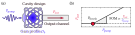
\includegraphics{figures/laser.png}}%%
    \caption{Topology optimization of nanolasers. (a) Working principle of a nanolaser. A pump with power $P_\text{pump}$ excites a gain medium with profile
    $D_0$ that emits a single lasing mode into an output channel with power $P_\text{out}$. (b) The optimization FOM is proportional to the linear relation between the pump and output power ($P_\text{out}/P_\text{pump}$),
    just above the lasing threshold ($P \gtrapprox P_\text{thres}$).  Adapted from~\cite{ownpub4}.}
    \label{fig:laser2d}
\end{figure}

To circumvent this, in~\cite{ownpub4} we propose a synthesis of SPA-SALT, perturbation theory, and coupled mode theory to simplify the problem. 
The two key results of this derivation are the expression of the lasing threshold and the FOM for the optimization, which can be evaluated by solving a linear system of equations.
The expression for the \textbf{lasing threshold}\footnote{To evaluate this expression still requires one eigensolve to determine $Q$.} is given by~\cite{ownpub4}
\begin{equation}\label{eq:pump_thresh}
 d_\text{thresh} = \frac{1}{\Gamma Q} = \frac{1}{Q} \frac{\int_{\Omega} \varepsilon_c(\mathbf{r})|\mathbf{E}_{\text{r}}(\mathbf{r})|^2\, \d \Omega}{\int_{\Omega} D_0(\mathbf{r}) |\mathbf{E}_{\text{r}}(\mathbf{r})|^2\, \d \Omega}\,.
\end{equation}
where $\mathbf{E}_\text{r}$ is the field in a reciprocal problem (\secref{sec:nanophotonics}) where the system is excited from an output port\footnote{In a high-$Q$ system, the field from the reciprocal solve $\mathbf{E}_r$ is almost exactly equal to the cavity mode and/or the lasing mode plus a $\mathcal{O}(1/\sqrt{Q})$ error~\cite{phot_crys}.} (e.g. the waveguide in \figref{fig:laser2d}), $Q$ is the quality factor of the cavity resonance, and $\Gamma$ is a measure 
of energy confinement in the gain region. From this expression, one can reduce the lasing threshold (for more energy-efficient lasers) by increasing $Q$ and enhancing the energy confinement in the
active medium ($\Gamma$). Note that in the single-emitter limit, where $D_0(\mathbf{r})\propto \delta (\mathbf{r}-\mathbf{r^\prime})$ for an emitter located at $\mathbf{r}^\prime$, this expression becomes $d_\text{thresh}=V/Q$, where $V$ is a measure
of the modal volume, a common FOM in other non-laser related inverse design works (e.g.,~\cite{LDOS_opt_wang}).

The second key result of the work is \textbf{a FOM for nanolaser design} that can also be evaluated through a single linear reciprocal solve~\cite{ownpub4}
\begin{equation}\label{eq:eff_nl}
    \frac{P_\text{out}}{P_\text{pump}} \propto \frac{\left( \int_{\Omega} D_0(\mathbf{r})|\mathbf{E}_{\text{r}}(\mathbf{r})|^2 \,  \d \Omega \right)^3} {\int_{\Omega} D_0(\mathbf{r}) |\mathbf{E}_{\text{r}}(\mathbf{r})|^4 \,  \d \Omega} = \text{FOM}.
\end{equation}
We refer to this FOM as the \emph{nonlinear} FOM, since it accounts for the laser nonlinearities perturbatively. The FOM is roughly proportional 
to the energy in the cavity ($\sim |\mathbf{E}_{\text{r}}|^6 / |\mathbf{E}_{\text{r}}|^4 \sim |\mathbf{E}_{\text{r}}|^2$), and thus to the $Q$ factor, which also contributes to attaining to a low
laser threshold (\eqref{eq:pump_thresh}). Consequently, as the optimization progresses, the high-$Q$ assumption in SPA-SALT (\eqref{eq:SPA_SALT}) will become more and more accurate. In the single emitter limit, the FOM becomes
$\text{FOM}=\vert \mathbf{E}_{r}(\mathbf{r}^\prime) \vert$, an
 LDOS-like FOM, which via reciprocity is proportional to the total power emitted into an output channel~\cite[App.~C]{reci}. Note that this FOM also describes the case of a single-point gain region (e.g., a quantum dot),
whose location is randomly distributed in the cavity with a probability density $\mathcal{P} \sim D_0$. 

To show how the nonlinear FOM compares to more conventional cavity-optimization approaches, we introduce a “naive” generalization of the LDOS, which heuristically modifies the definition
of the LDOS to account for out-coupling efficiency [through a reciprocal solve ($\mathbf{E}_r$)] and a distributed gain
medium $D_0$
\begin{equation}\label{eq:SEL}
 \text{FOM}_{\text {naive }}=\int_{\Omega} D_0(\mathbf{r})\left|\mathbf{E}_{\text{r}}(\mathbf{r})\right|^2 \d \Omega\,,
\end{equation}
which we refer to as the \emph{naive} FOM, defined by the overlap of the electric-field intensity of the reciprocal field with the gain distribution.
Note that this naive FOM is also proportional to the intensity of the reciprocal field ($\sim |\mathbf{E}_{\text{r}}|^2$), and thus roughly proportional to $Q$, thus ensuring 
high-$Q$ optimized cavities.

\subsection*{Optimization results for extended gain media}

\begin{figure}[tb]
    \centering
    \makebox[\textwidth][c]{\includegraphics{figures/laser_size.png}}%%
    \caption{Performance of the topology-optimized devices for the nonlinear and naive FOMs for different Gaussian gain distributions with standard deviations $\sigma_g$. (a) Device optimize for a point-like gain region ($\sigma_g=25$ nm).
    (b) Device optimized for $\sigma_g=250$ nm. (c) Device optimized for $\sigma_g=500$ nm. Adapted from~\cite{ownpub4}.}
    \label{fig:laser_size}
\end{figure}

Using this formalism, we optimize two-dimensional nanolasers and study the influence of the gain region size in 
nanolaser design (\figref{fig:laser_size}). A design-dependent Gaussian distribution describes the gain medium, 
\begin{equation}
D_0 (\mathbf{r}, \hat{\rho}) = \varepsilon_{\text{r}}(\mathbf{r})  \hat{\rho}(\mathbf{r}) \, e^{- \vert \mathbf{r} - \mathbf{r}_0 \vert^2 / 2 \sigma_{\text{g}}^2 }
\end{equation}
, where
$\sigma_g$ is the standard deviation of the Gaussian and acts as a measure of the gain region size. We verify that for point-like gain regions, the devices optimized for the FOM and the naive FOM (\eqref{eq:SEL})
achieve similar performance (limited by the finite size of the tiny gain region), favoring bowtie-like cavity designs
where the in-plane electric field is concentrated at a bowtie sharpness-limited field singularity~\cite{sing}. Moreover, we show that for
distributed gain media with sizes comparable to the wavelength ($\sigma_g \sim \lambda$, for $\lambda=1.55$ \textmu m) the derived FOM discourages field localization due to the denominator in \eqref{eq:eff_nl} (since $\int \vert \mathbf{E} \vert^2$ is finite), in contrast to the naive FOM, 
resulting in a $\approx 3\times$ enhancement when targeting the correct nanolaser FOM (\eqref{eq:eff_nl}). 
\subsection*{Accounting for gain diffusion}

In semiconductors with extended gain media, it is essential to model the electrical effect of \textbf{carrier diffusion}. This effect can be introduced by modeling the semiconductor gain medium in the free-carrier approximation\footnote{Neglecting carrier-carrier Coulomb interactions.}, using a diffusion 
equation~\cite{csalt}. Using this formalism, we re-derive the expression for the lasing threshold (\eqref{eq:pump_thresh}) when accounting for carrier diffusion~\cite{ownpub4}, where the lasing threshold is
\begin{equation}\label{eq:pump_thresh_diff}
 d_\text{thresh} = \frac{1}{Q} \frac{\int_{\Omega} \varepsilon_c(\mathbf{r})|\mathbf{E}_{\text{m}}(\mathbf{r})|^2\, \d \Omega}{\int_{\Omega} \mathbb{S} [D_0] (\mathbf{r}) |\mathbf{E}_{\text{m}}(\mathbf{r})|^2\, \d \Omega}\,,
\end{equation}
and the nanolaser FOM (\eqref{eq:eff_nl}) with carrier diffusion effects is
\begin{equation}\label{eq:eff_diff}
 \text{FOM} =  \frac{\left(\int_{\Omega} \mathbb{S} [D_0](\mathbf{r}) |\mathbf{E}_{\text{r}}(\mathbf{r})|^2 \, \d \Omega\right)^3} {\int_{\Omega} \mathbb{S}\left[ |\mathbf{E}_{\text{r}}|^2\, \mathbb{S} [D_0] \right] (\mathbf{r})|\mathbf{E}_{\text{r}}(\mathbf{r})|^2 \, \d \Omega}\,.
\end{equation}
These expressions use the diffusion operator $\mathbb{S}^{-1}= \mathbb{I}+\nabla \cdot (R_\nabla^2(\mathbf{r}) \nabla)$, where $\mathbb{I}$ is the identity operator, and $R_\nabla (\mathbf{r})$ is a diffusion lengthscale determined by the spatially- and design-dependent diffusion coefficient.
In this notation, computing $u = \mathbb{S}[b]$ corresponds to solving for the scalar field $u$ in the diffusion problem $\mathbb{S}^{-1}u=b$, where $b$ is a scalar field. 
The main difference when accounting for diffusion is that now one needs to consider the profile of diffused carriers ($\mathbb{S} [D_0]$) in the lasing threshold (\eqref{eq:pump_thresh_diff}), and the diffusion of the gain depletion ($\mathbb{S}[ |\mathbf{E}_{\text{r}}|^2\, \mathbb{S} [D_0]]$)
in the FOM denominator (\eqref{eq:eff_diff}). Note that in the small diffusion limit ($R_\nabla \ll \lambda, \mathbb{S} \approx \mathbb{I}$)
we recover the original expressions in \eqref{eq:pump_thresh} and \eqref{eq:eff_nl}.

\begin{figure}[tb]
    \centering
    \makebox[\textwidth][c]{\includegraphics{figures/laser_carriers.png}}%%
    \caption{Topology-optimized devices with gain diffusion effects for a gain region with size $\sigma_g=250$ nm and a diffusion length of $R_\nabla=5$ \textmu m. The device optimized without accounting for gain diffusion ("Nonlinear FOM") and the device optimized accounting for gain diffusion ("Diffusion FOM") have the gain profile $D_0$ that is diffused ($\mathbb{S}[D_0]$)
    in the semiconductor-like material, generating the optical field given by the electric-field norm $\vert \mathbf{E} \vert$. Adapted from~\cite{ownpub4}.}
    \label{fig:laser_diff}
\end{figure}

By using the expression in \eqref{eq:eff_diff} as an optimization FOM, we study how accounting for diffusion effects
affects nanolaser designs and performance. As shown in \figref{fig:laser_diff}, the device that accounts for diffusion disconnects the cavity from the waveguide while also removing
material from areas of weak electric field to 
enhance the coupling between the carriers and the optical field, and results in a $\approx 2\times$ enhancement when considering the diffusion-corrected FOM. 

\subsection*{Towards realizable nanolasers: three-dimensional designs}

Finally, we apply the formalism to design three-dimensional silicon-on-insulator nanolasers (\figref{fig:laser3d}), 
and verify that, similar to the two-dimensional case, the FOM discourages field localization while still efficiently coupling to the output waveguide, yielding a $\approx 1.6\times$
enhancement when considering the correct nonlinear FOM for extended gain media (\eqref{eq:eff_nl}). We attribute the enhancement drop with respect to the two-dimensional optimization results to the fact that localizing a high-$Q$ resonance is more difficult in three dimensions.

\begin{figure}[tb]
    \centering
    \makebox[\textwidth][c]{\includegraphics{figures/laser_2.png}}%%
    \caption{Topology-optimized nanolasers in three dimensions. The devices lases into the cavity mode (inset plot) and out-couple to the waveguide mode. (a) Device optimized for the naive FOM. (b) Device optimized for the nonlinear FOM.
    Adapted from~\cite{ownpub4}.}
    \label{fig:laser3d}
\end{figure}

\subsection*{Outlook and future work}

In conclusion, in \cite{ownpub4} we show that by exploiting perturbative analysis valid in high-$Q$ cavities, one can derive  
an efficient FOM for laser performance ($\propto P_\text{out}/P_\text{pump}$) that captures resonant enhancement,  
spatial hole-burning, and gain diffusion at little extra computational cost. The FOM evaluation requires only a  
single linear reciprocal Maxwell solve (plus potentially two scalar solves for gain diffusion), making it 
an efficient formulation for laser optimization. This efficient first-principles approach allows for inverse nanolaser design in two and three dimensions, while  
also allowing for future refinements, including accounting for the laser linewidth~\cite{pick}, or accurate pumping models, where optical or electrical pumping could be explicitly
modeled.

\openright
\chapter{Concluding remarks}

This thesis presents a comprehensive study on multiphysics topology optimization in nanophotonics, focusing on developing novel design
methods for applications that rely on coupled physical effects, such as thermo-optical, optomechanical, and electro-optical interactions.

We begin by introducing the field of nanophotonics (\secref{sec:nanophotonics}) and the numerical solution of Maxwell's equations
(\secref{sec:fem}), which form the foundation for single-physics topology optimization. We then extend the framework to multiphysics
problems (\secref{sec:coupled}) and present a general multiphysics topology optimization formulation (\secref{sec:topopt_theory}).

Next, we address thermo-optical topology optimization (\chapref{chap:eo}), focusing on designing low-loss phase shifters
 (\secref{sec:TOPS}) by optimizing metallic heater layouts around optical waveguides. We derive the first coupled multiphysics topology optimization formulation
in the nanophotonics literature and demonstrate compact, efficient conduction heater designs that reduce optical losses by
$\approx 33\%$ compared to state-of-the-art solutions.

We then explore optomechanical topology optimization (\chapref{chap:om}). First, we optimize the design of particles and their environments for optical force engineering (\secref{sec:engi}) by developing a topology optimization framework that uses the MST formalism to target optical forces on particles of arbitrary size and shape.
Our optimized designs show that tailoring both the particle geometry and its
environment can significantly enhance momentum exchange with an optical field, achieving force enhancements of up to
$\approx 13\times$ compared to a reference design. Next, we design integrated photonic cavities for sub-wavelength particle trapping
(\secref{sec:dip}) and theoretically demonstrate omnidirectional trapping without relying on SIBA effects, while achieving a trapping stiffness
an order of magnitude larger than that of diffraction-limited optical tweezers. Lastly, we optimize optomechanical membranes
(\secref{sec:mech_strongly_coupled}) whose optical response strongly couples to mechanical deformation. By accounting for
optical-force-induced deformation in the design, we achieve a performance improvement of $\approx 3\times$ over designs that
neglect this effect, highlighting the importance of including multiphysics interactions in the design process.

Finally, we consider electro-optical topology optimization (\chapref{chap:eo}), where we derive an efficient formulation for nanolaser design
(\secref{sec:laser}). We apply this approach to design two- and three-dimensional nanolasers and show that using
 a laser physics-based FOM (accounting for factors such as extended gain media and steady-state diffusion) outperforms
  heuristic local-density-of-states-like metrics, yielding up to a $\approx 3\times$ improvement.

Overall, this research contributes to the design of novel nanophotonic devices that leverage multiphysics interactions, enabling enhanced functionality, improved performance, and new capabilities in nanophotonic systems.

\section{Future work}

This work opens several avenues for future research, including:

\begin{itemize}
    \item \textbf{Application to experimental setups:} While the framework was developed theoretically, it can be adapted to specific experimental configurations with minor, problem-dependent modifications.
    
    \item \textbf{Nonlinear multiphysics extensions:} The current adjoint formulation (\secref{sec:topopt_theory}) handles cascaded nonlinear dependencies in coupled systems, where the couplings are nonlinear but physics system can still be solved linearly. Future work could extend this to fully nonlinear systems, where each governing equations depend on their respective state solution.
    
    \item \textbf{Simultaneous multiphysics effects:} Extending the framework to handle multiple coupled effects, such as thermo-electro-optical interactions or combined geometric deformation and photoelasticity (\secref{sec:mech_strongly_coupled}), could unlock advanced device functionalities.
    
    \item \textbf{Advanced figures of merit (FOMs):} More sophisticated FOMs could be developed to better capture relevant physical effects. As an example, in the optical force engineering problem (\secref{sec:engi}), one could target optical torque (\eqref{eq:torque}) or design the spatial distribution of forces for engineered particle motion.
    
    \item \textbf{Strongly coupled systems:} Beyond the optomechanical membrane problem studied in~\secref{sec:mech_strongly_coupled}, other strongly coupled problems, like heat-induced refractive index changes from optical absorption (\secref{sec:thermo_strong_coupling}), could be investigated.
    
    \item \textbf{Nanolaser pumping models:} The nanolaser topology optimization framework (\secref{sec:laser}) could be extended to include explicit models of optical or electrical pumping.
\end{itemize}

\newrefcontext[labelprefix=]
\sloppy
\printbibliography[notkeyword=myPub,notkeyword=myMan]


\appendix
\chapter{Appendix}
\section{Adjoint sensitivity analysis in coupled mutliphysics problems -- sequential and parallel coupling}\label{app:appendix1}

In this appendix we derive the expressions for the adjoint sensitivity analysis in seggregatedly coupled multiphysics problems.
 This means that the coupling is unidirectinal, so that $\mathbf{u}_1 \to \mathbf{u}_2$ and $\mathbf{u}_1 \not\to \mathbf{u}_2$, for two
 coupled state fields $\mathbf{u}_1$ and $\mathbf{u}_2$. For simplicity, we consider
only real fields. We also restrict ourselves to coupling through material properties (Sec. XX), but this can be extended to other couplings
(e.g., source terms, Sec. YY).\\

In the most general case of $N$ coupled physics problems we can rewrite the FOM by adding the residual
of the state equations, multiplied by the Lagrange multipliers, $\lambda_i$, 
respectively:
\begin{equation}\label{eq:adj_init}
    \tilde{\Phi} =\Phi + \sum^N_i \lambda_{i}^{\top}\left(\mathbf{S}_i \mathbf{u}_i -\mathbf{f}_i\right)\,.
\end{equation}
Now we will see how this can be used to calculate the sensitivities when the physics are coupled in a sequential or parallel way.

\subsection{Sequential coupling}

In the sequential case, the solutions of the different physics couple one-to-one in a seggregated fashion (
$\mathbf{u}_1 \to \mathbf{u}_2 \to \cdots \to \mathbf{u}_N$)
and there is no other coupling mechanism between the physics. In this case, taking the derivative of the FOM with respect to the design variable $\xi$:
\begin{equation}\label{eq:adj_seq}
    \frac{\d \tilde{\Phi}}{\d \xi} = \frac{\partial \Phi}{\partial \xi} + \mathcal{D}^{(1)}_\circ \left[\Phi\right] + 
    \sum^N_i \lambda_{i}^{\top} \left[ \left(\frac{\partial \mathbf{S}_i}{\partial \xi} +  \mathcal{D}^{(i)}_\circ \left[\mathbf{S}_i\right]\right) \mathbf{u}_i
    + \mathbf{S}_i \mathcal{D}^{(i)}_\circ \left[\mathbf{u}_i\right] - \frac{\partial \mathbf{f}_i}{\partial \xi }\right]
\end{equation}
where we have defined $\mathcal{D}^{(i)}_\circ[a]$ as the sequential or composition ($\circ$) differential operator acting on $a$ to compactly write the derivative:
\begin{align}
    \mathcal{D}^{(i)}_\circ[a] &= \frac{\partial a}{\partial \mathbf{u}_i} \sum_{j=i}^{N} \frac{\partial \mathbf{u}_j}{\partial \xi} 
        \prod_{k \leq j}^{j} \frac{\partial \mathbf{u}_k}{\partial \mathbf{u}_{k+1}}\,, \\
        &= \frac{\partial a}{\partial \mathbf{u}_i} \left( \frac{\partial \mathbf{u}_i}{\partial \xi} + 
            \frac{\partial \mathbf{u}_i}{\partial \mathbf{u}_{i+1}} \left( \frac{\partial \mathbf{u}_{i+1}}{\partial \xi} + 
                \frac{\partial \mathbf{u}_{i+1}}{\partial \mathbf{u}_{i+2}} \left( \frac{\partial \mathbf{u}_{i+2}}{\partial \xi} + 
                    \cdots
                \right)
            \right)
        \right) \,.
    \end{align}
Using Eq.~\eqref{eq:adj_seq} and grouping the terms:
\begin{equation}
    \frac{\d \tilde{\Phi}}{\d \xi} =  \frac{\partial \Phi}{\partial \xi} + \sum_i \lambda_{i}^{\top} \left( \frac{\partial \mathbf{S}_i}{\partial \xi} \mathbf{u}_i - \frac{\partial \mathbf{f}_i}{\partial \xi} \right)
    + \sum^{N-1}_{i=1}  \frac{\partial \mathbf{u}_{i}}{\partial \xi} \left( \lambda_{i}^{\top} \frac{\partial \mathbf{S}_i}{\partial \mathbf{u}_{i+1}}\mathbf{u}_{i}
    +  \lambda_{i+1}^{\top} \mathbf{S}_{i+1}\right)\,.
\end{equation}
We can by choose the Lagrange multipliers to the last summation term is zero, by solving $N$ adjoint equations:
\begin{align}
    \mathbf{S}^\top_{1}\lambda_{1} &= - \frac{\partial \Phi}{\partial \mathbf{u}_{1}} \label{eq:seq_adj_1}\,\\
    \mathbf{S}^\top_{i+1}\lambda_{i+1} &= - \mathbf{u}^\top_i \left(\frac{\partial \mathbf{S}_i}{\partial \mathbf{u}_{i+1}}\right)^\top \lambda_i \quad \forall i \in [1, N-1] \label{eq:seq_adj_N-1}\,,
\end{align}
where the adjoint equations imply a relationship where the coupling happens backwards. In other words, one needs to solve the first adjoint equation (Eq.~\eqref{eq:seq_adj_1}), 
and feed the solution the next adjoint equation ($i=2$, Eq.~\eqref{eq:seq_adj_N-1}) (and so on); where the coupling is inverted with respect to the physics. Solving these adjoint equations we can calculate the lagrang
multipliers which give the final sensitivities:
\begin{equation}
    \frac{\d \tilde{\Phi}}{\d \xi} = \frac{\partial \Phi}{\partial \xi} + \sum_i \lambda_{i}^{\top} \left( \frac{\partial \mathbf{S}_i}{\partial \xi} \mathbf{u}_i - \frac{\partial \mathbf{f}_i}{\partial \xi} \right)\,.
\end{equation}

\subsection{Parallel coupling}

Let's now consider the case of parallel coupling, where the solution of $N-1$ physics are coupled solve the last ($i=1$) physics ($[\mathbf{u}_2, \mathbf{u}_3, \cdots, \mathbf{u}_{N-1}] \to \mathbf{u}_1$). By reusing Eq.~\eqref{eq:adj_seq},
we can now take the derivative with respect to the design variables:
\begin{align}\label{eq:adj_parallel}
    \frac{\d \tilde{\Phi}}{\d \xi} &= \frac{\partial \Phi}{\partial \xi} + \mathcal{D}^{(1)}_\parallel \left[\Phi\right]  
    +  \lambda_{1}^{\top} \left[\left( \frac{\partial \mathbf{S}_1}{\partial \xi} +  \mathcal{D}^{(1)}_\parallel \left[\mathbf{S}_1\right] \right) \mathbf{u}_1
    + \mathbf{S}_1  \mathcal{D}^{(1)}_\parallel \left[\mathbf{u}_1\right] \right] + \\
    &+ \sum_{i=2}^{N} \lambda_{i}^{\top} \left( \frac{\partial \mathbf{S}_i}{\partial \xi}\mathbf{u}_i + \mathbf{S}_i \frac{\partial \mathbf{u}_i}{\partial \xi} - \frac{\partial \mathbf{f}_i}{\partial \xi}\right)
\end{align}
where we have defined $\mathcal{D}^{(i)}_\parallel[a]$ as the parallel ($\parallel$) differential operator acting on $a$ to compactly write the derivative:
\begin{equation}
    D^{(i)}_\parallel[a] = \frac{\partial a}{\partial \mathbf{u}_i} \sum_{j=1}^{N} \frac{\partial \mathbf{u}_j}{\partial \mathbf{u}_i} 
    \frac{\partial \mathbf{u}_j}{\partial \xi}\,.
\end{equation}
Using Eq.~\eqref{eq:adj_parallel} and grouping the terms:
\begin{equation}
    \frac{\d \tilde{\Phi}}{\d \xi} = \frac{\partial \Phi}{\partial \xi} + \sum_i \lambda_{i}^{\top} \left( \frac{\partial \mathbf{S}_i}{\partial \xi} \mathbf{u}_i - \frac{\partial \mathbf{f}_i}{\partial \xi} \right)
    + \frac{\partial \mathbf{u}_1}{\partial \xi} \left( \lambda_{1}^{\top}  \mathbf{S}_1 + \frac{\partial \Phi}{\partial \mathbf{u}_1} \right) + 
    \sum^{N}_{i=2} \left( \lambda_{i}^{\top} \mathbf{S}_i + \lambda_{1}^{\top}  \frac{\partial \mathbf{S}_i}{\partial \mathbf{u}_1} \mathbf{u}_i\right)\,.
\end{equation}
We can by choose the Lagrange multipliers so that the last two terms are zero, by solving $N$ adjoint equations:
\begin{align}
    \mathbf{S}^\top_{1}\lambda_{1} &= - \frac{\partial \Phi}{\partial \mathbf{u}_{1}} \label{eq:par_adj_1}\,\\
    \mathbf{S}^\top_{i}\lambda_{i} &= - \mathbf{u}^\top_1 \left(\frac{\partial \mathbf{S}_1}{\partial \mathbf{u}_i}\right)^\top \lambda_1 \quad \forall i \in [2, N] \label{eq:par_adj_N-1}\,,
\end{align}
The Lagrange multipliers are a solution to this equation and can be used to simplify the sensitivity expression:
\begin{equation}
    \frac{\d \tilde{\Phi}}{\d \xi} = \frac{\partial \Phi}{\partial \xi} + \sum_i \lambda_{i}^{\top} \left( \frac{\partial \mathbf{S}_i}{\partial \xi} \mathbf{u}_i - \frac{\partial \mathbf{f}_i}{\partial \xi} \right)\,.
\end{equation}
which is the same result as in the case of sequential coupling, with different Lagrange multipliers.

\subsection{Generalizing to simultaenous sequential and parallel coupling}
Based on the result from the previous sections, in the general coupling case, where there might be parallel and sequential couplings simultaneously, the sensitivities can be calculated as:
\begin{equation}
    \frac{\d \tilde{\Phi}}{\d \xi} = \frac{\partial \Phi}{\partial \xi} + \sum_i \lambda_{i}^{\top} \left( \frac{\partial \mathbf{S}_i}{\partial \xi} \mathbf{u}_i - \frac{\partial \mathbf{f}_i}{\partial \xi} \right)\,.
\end{equation}
The only difference is solution to the adjoint equations, which depends on the coupling. In the general case, where all couplings feed to a 
final physics ($i=1$) but may be coupled in any combinations between each other, it can be shown that the adjoint equations are:
\begin{align}
    \mathbf{S}^\top_{1}\lambda_{1} &= - \frac{\partial \Phi}{\partial \mathbf{u}_{1}}\,\\
    \mathbf{S}^\top_{i}\lambda_{i} &= - \sum^{C_i}_j \mathbf{u}^\top_j \left(\frac{\partial \mathbf{S}_j}{\partial \mathbf{u}_{i}}\right)^\top \lambda_j \quad \forall i \in [1, N-1]\, , \quad \forall j \in [1, C_i] \,.
\end{align}
where $C_i<N$ is the number of physics that are coupled to the $i$th physics, and where we have used that the problems are linear. 
Note that the couplings are still unidirectional. To extend this derivations to complex fields one can refer to the adjoint sensitivity
analysis in \cite{ownpub0}, for a simpler two-physics ($N=2$) problem, where the optical problem uses complex fields.



\pagestyle{plain}

\FloatBarrier
\chapter*{Publications}
\addcontentsline{toc}{chapter}{Publications}%
\vspace*{0.4\textheight}
\begin{center}
  \begin{minipage}{0.9\linewidth}
    \section*{Publication \cite{ownpub0}}
    \addcontentsline{toc}{section}{Publication \cite{ownpub0}}%
    Beñat Martinez de Aguirre Jokisch, Rasmus Ellebæk Christiansen, and Ole Sigmund, "Topology optimization framework for designing efficient thermo-optical phase shifters," J. Opt. Soc. Am. B 41, A18-A31 (2024).
  \end{minipage}
\end{center}
\newpage
\includepdf[pages=-,width=1.005\paperwidth, templatesize={\paperwidth}{\paperheight}, offset=1mm -0.7mm]{ownPub/ownpub0.pdf}

\vspace*{0.4\textheight}
\begin{center}
  \begin{minipage}{0.9\linewidth}
    \section*{Publication \cite{ownpub1}}
    \addcontentsline{toc}{section}{Publication \cite{ownpub1}}%
    Beñat Martinez de Aguirre Jokisch, Benjamin Falkenberg Gøtzsche, Philip Trøst Kristensen, Martijn Wubs, Ole Sigmund, and Rasmus Ellebæk Christiansen, "Omnidirectional Gradient Force Optical Trapping in Dielectric Nanocavities by Inverse Design," ACS Photonics 11 (12), 5118-5127 (2024).
  \end{minipage}
\end{center}
\newpage
\includepdf[pages=-,width=1.005\paperwidth, templatesize={\paperwidth}{\paperheight}, offset=1mm -0.7mm]{ownPub/ownpub1.pdf}

\vspace*{0.4\textheight}
\begin{center}
  \begin{minipage}{0.9\linewidth}
    \section*{Publication \cite{ownpub3}}
    \addcontentsline{toc}{section}{Publication \cite{ownpub3}}%
    Beñat Martinez de Aguirre Jokisch, Ole Sigmund, and Rasmus Ellebæk Christiansen, "Inverse design of dielectric nanostructures for optical trapping,"  Proc. SPIE 13112, Optical Trapping and Optical Micromanipulation XXI, 1311204 (2024).
  \end{minipage}
\end{center}
\newpage
\includepdf[pages=-,width=1.005\paperwidth, templatesize={\paperwidth}{\paperheight}, offset=1mm -0.7mm]{ownPub/ownpub3.pdf}

\vspace*{0.4\textheight}
\begin{center}
  \begin{minipage}{0.9\linewidth}
    \section*{Publication \cite{ownpub2}}
    \addcontentsline{toc}{section}{Publication \cite{ownpub2}}%
    Beñat Martinez de Aguirre Jokisch, Rasmus Ellebæk Christiansen, and Ole Sigmund, "
    Engineering optical forces through Maxwell stress tensor inverse design,"  J. Opt. Soc. Am. B 42, 731-741 (2025).
  \end{minipage}
\end{center}
\newpage
\includepdf[pages=-,width=1.005\paperwidth, templatesize={\paperwidth}{\paperheight}, offset=1mm -0.7mm]{ownPub/ownpub2.pdf}

\vspace*{0.4\textheight}
\begin{center}
  \begin{minipage}{0.9\linewidth}
    \section*{Publication \cite{ownpub4}}
    \addcontentsline{toc}{section}{Publication \cite{ownpub4}}%
    Beñat Martinez de Aguirre Jokisch, Alexander Cerjan, Rasmus Ellebæk Christiansen, Jesper Mørk, Ole Sigmund, Steven G. Johnson, "
    Efficient first-principles inverse design of nanolasers,"  \textit{Submitted manuscript} (2025).
  \end{minipage}
\end{center}
\newpage
\includepdf[pages=-,width=1.005\paperwidth, templatesize={\paperwidth}{\paperheight}, offset=1mm -0.7mm]{ownPub/ownpub4.pdf}

%\vspace*{0.4\textheight}
%\begin{center}
%  \begin{minipage}{0.9\linewidth}
%    \section*{Manuscript \cite{ownpub1}}
%    \addcontentsline{toc}{section}{Manuscript \cite{ownpub1}}%
%    Bla bla bla...
%  \end{minipage}
%\end{center}
%\newpage
%\includepdf[pages=-,width=1.005\paperwidth, templatesize={\paperwidth}{\paperheight}, offset=1mm -0.7mm]{ownPub/ownpub1.pdf}



\cleardoublepage

\thispagestyle{empty}
\movetoevenpage
% Include back page here
\includepdf[pages=-,width=1\paperwidth, templatesize={\paperwidth}{\paperheight}, offset=0 -0.2mm]{Cover/Back.pdf}




\end{document}
